%\documentclass[10pt,twocolumn]{article}
\documentclass[11pt]{article}

\usepackage{graphicx}% Include figure files
\usepackage{setspace}
\usepackage{dcolumn}% Align table columns on decimal point
\usepackage{bm}% bold math
\usepackage{amsmath}
\usepackage{hyperref}
\usepackage{caption}
\usepackage{listings}
\usepackage{float}
\providecommand{\e}[1]{\ensuremath{\times 10^{#1}}}

\linespread{1.0}

\begin{document}

\title{Gpvdm manual}

\author{Roderick C. I. MacKenzie}


\maketitle




\centerline{roderick.mackenzie@nottingham.ac.uk}


\begin{figure}[ht!]
\centering
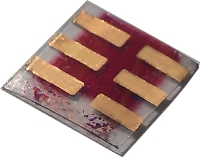
\includegraphics[width=30mm]{./images/cell.jpg}
\label{overflow}
\end{figure}

\newpage
\section{Foreword}
This manual is a work in progress, as people ask questions to do with gpvdm, I write the answer in the manual and then send the link to them.  So the text is far from exhaustive.  If something is not clear, just drop me an e-mail.  I also suggest you also read the papers which were published from this model - do also read the supplementary information (SI) to the papers, as I often write about the model in there.

\section{Running the model}

\subsection{Installing gpvdm for windows}
Go to the download page for gpvdm at \url{http://www.gpvdm.com/windows.php} and download the latest version.  Simply double click on it and say yes to all questions.  The installer may offer you a choice of where to install the software to, don't change the install destination, the current version will only work if it is in the default install path which is C:$\backslash$gpvdm.  I publish a new exe with updates every couple of weeks, however it is possible I won't actually use gpvdm for a while after having published a new version.  Therefore, it is entirely possible that I may have introduced bugs that break the code in between releases.  So, if gpvdm is not working for, you drop me an e-mail and I will do my best to fix it asap.

\subsection{Installing gpvdm for linux}
This is discussed in section \ref{installing_on_linux}.

\section{Running gpvdm}
On both windows and linux gpvdm will install on the start menu, click on it to launch it.  Once run, a window resembling that in figure \ref{fig:mainwindow} will appear.  From the left, the first three icons on the toolbar, open a simulation, save a simulation and generate a new simulation.  Once you have made a new simulation, the the play button will run it, and the stop button will stop the simulation running.  You will find more video examples describing how to use the model throughout the gpvdm web page.

\begin{figure}[ht!]
\centering
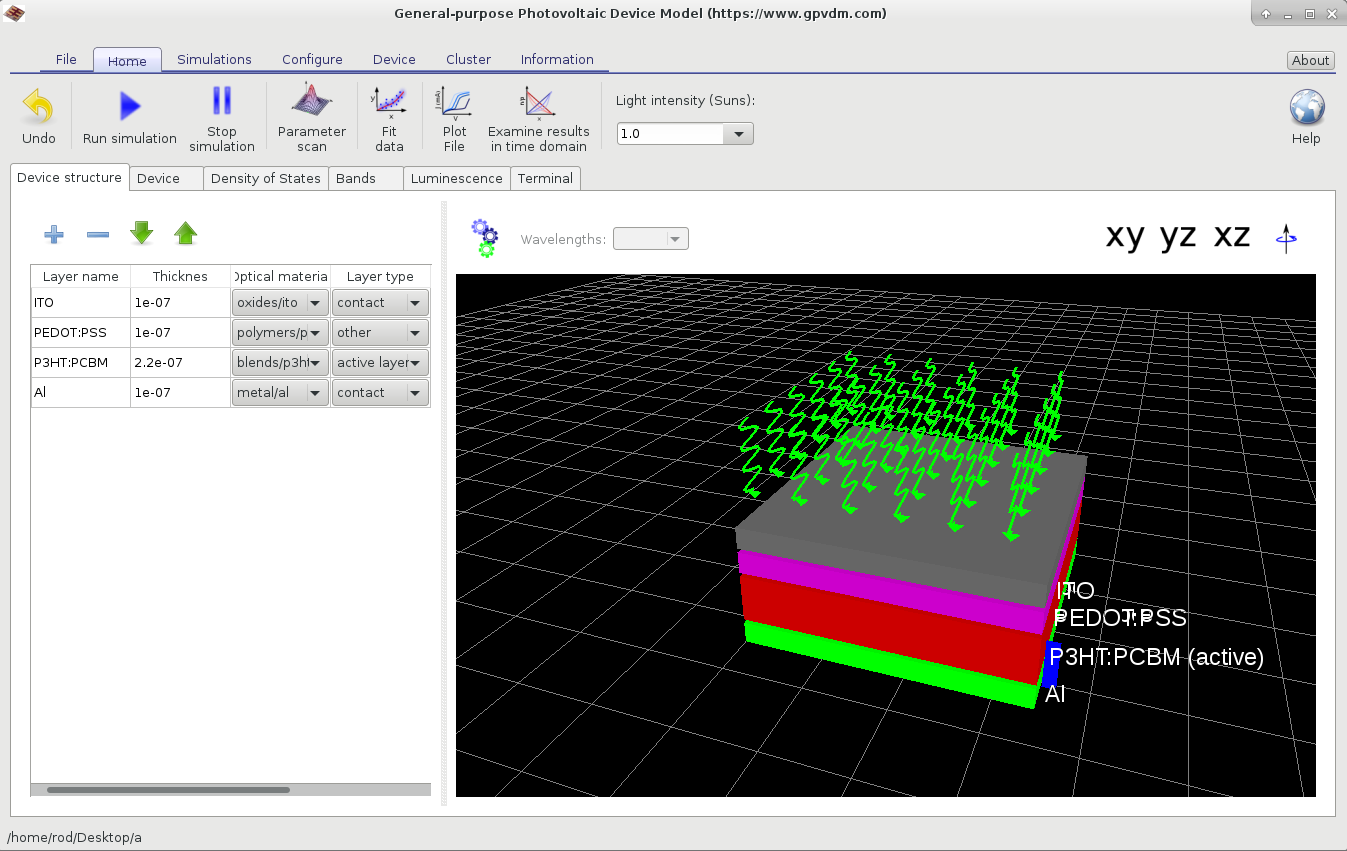
\includegraphics[width=140mm]{./images/main_window.png}
\caption{The main window, with a picture of the device on the right and the layer editor on the left.}
\label{fig:mainwindow}
\end{figure}

Each set of model parameters is displayed in an individual simulation tab.  For example the tab 'DoS layer' contains the material parameters for material layer 0.  These include mobility, recombination cross sections, tail slopes and band gaps.  The 'device' tab is used to set information about the device, such as shunt resistance, series resistance and density of electrons/holes on the contacts.

\subsection{Meshing}
\subsubsection{Editing the electrical mesh/layers}
The device structure is split up into layers of different materials.  These can be configured in layer editor.  Some of these layers will have the layer type 'active'.  An 'active' layer is a layer over which the electrical model will be applied.  The electrical model needs a finite difference mesh to to be setup for it to work.  Usually, this will be take care of automatically, by gpvdm.  However, some users will want fine control over the mesh.  The electrical mesh editor is depicted in figure \ref{fig:emesh}.


The buttons marked 1D, 2D and 3D at the top of the window can be used to toggle the simulation between 1D, 2D and 3D modes.  (Note, if you want to do 2D or 3D simulations you are best off using a default 2D simulation, such as the OFET simulation.  This is because to do 2D/3D simulations, a special newton solver configuration will be needed.) The table on the left hand side is used to configure the mesh.  The sum of the mesh layer thicknesses must exactly match that of the sum of the active layers.  If this is not the case, the model will automatically rewrite the electrical mesh, to something that has the correct dimensions but may not be what the user desires.  Automatic mesh configuration can be turned off though the cog icon.  The columns thickness and mesh points, determine the thickness of the mesh layer and the number of points on the mesh layer, if there is a uniform spacing between mesh points.  The column, 'step multiply' by how much to grow each step.  In this example, the mesh spacing is increased by a factor of 0.1 each step.  The toggle button left/right, defines on which side the mesh layer is generated.  In this example there are two mesh layers, one starting on the left and one starting on the right.  The resulting mesh is plotted in the graph at the bottom of the window.  It can be seen that a non-linear mesh has been generated.

\begin{figure}[ht!]
\centering
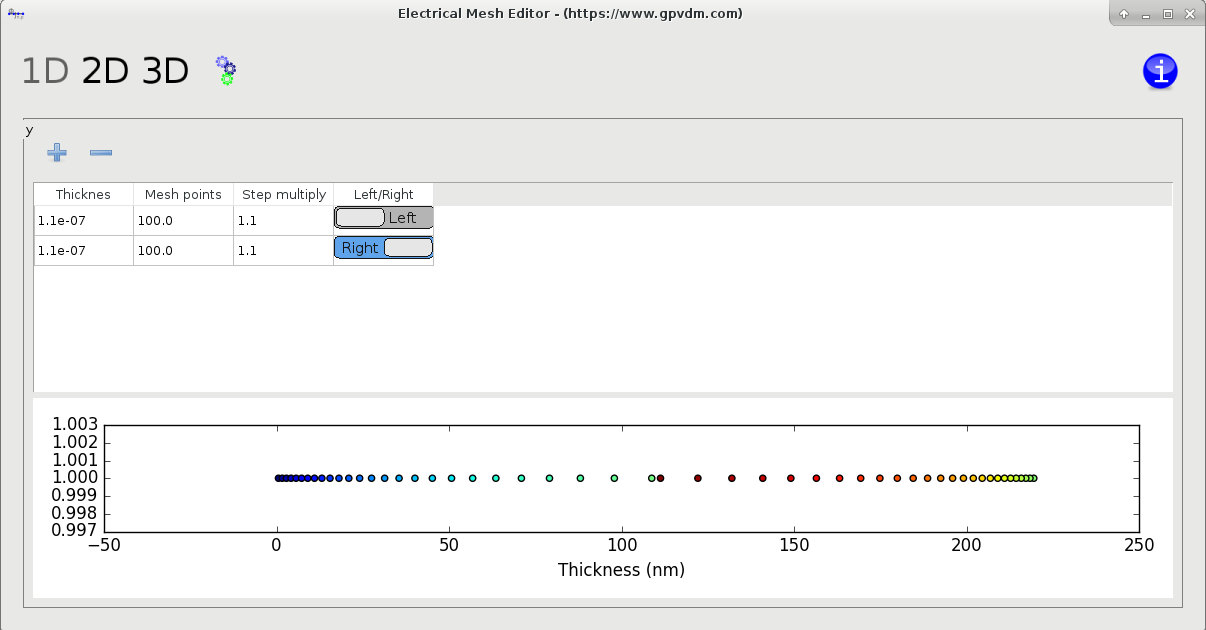
\includegraphics[width=140mm]{./images/emesh.png}
\caption{The electrical mesh editor}
\label{fig:emesh}
\end{figure}

\begin{figure}[ht!]
\centering
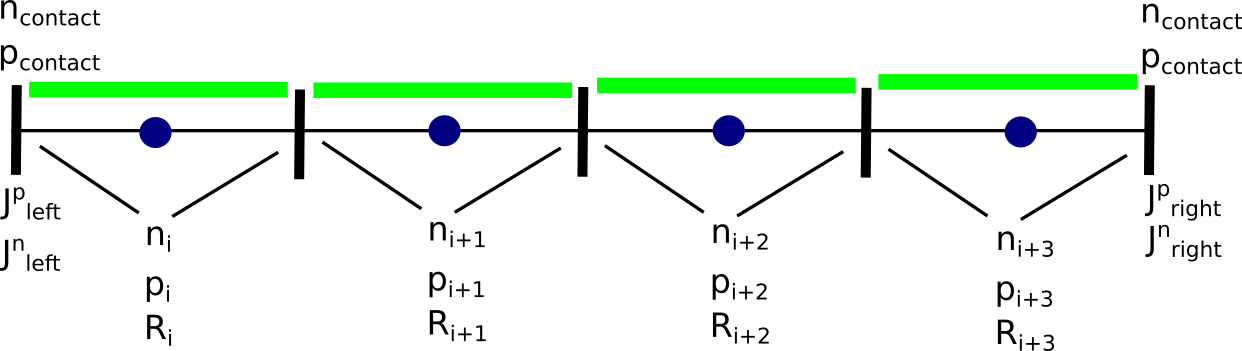
\includegraphics[width=140mm]{./images/mesh.png}
\caption{A 1D diagram of the mesh}
\label{fig:emeshdiagram}
\end{figure}


\subsubsection{Editing the optical mesh/layers}
The optical mesh automatically extends to cover the optical simulation window, so one does not usually need to worry about configuring it.  The optical material layers are defined in the list at the bottom of figure \ref{fig:emesh}.  The first column is a unique identifier, it must start with a hash symbol, but apart from that you can call it what you want.  The second column is the thickness of the layer.  The forth column is the material system, data files describing the material system are stored in the 'phys' directory.  Finally, the forth column tells the model if the layer is part of the active layer or not (more about that in the next section.)

\begin{figure}[ht!]
\centering
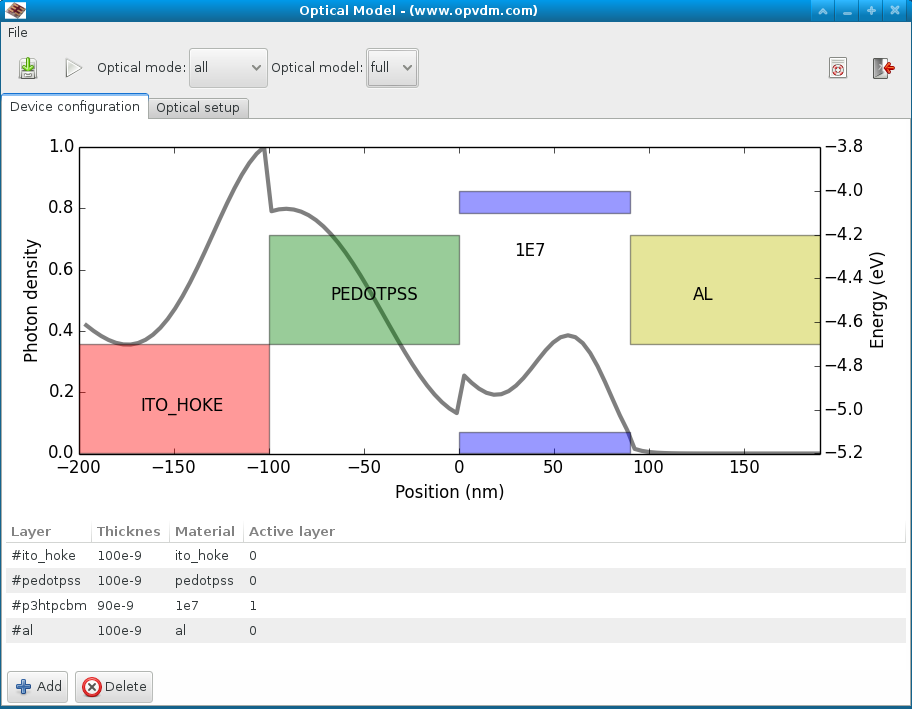
\includegraphics[width=140mm]{./images/opticalsimulation.png}
\caption{The electrical mesh editor}
\label{fig:opticalsimulation}
\end{figure}

\subsubsection{Interfacing the electrical and optical models}
In gpvdm there is both an electrical model and an optical model.  The optical simulation usually includes the glass substrate, the contacts and layers such as PEDOT:PSS.  The electrical simulation usually only covers the active layer of the device, thus a typically optical simulation is much bigger than the electrical simulation window.  The optical model feeds the calculated optical profile of the light into the electrical simulation.  You must therefore tell the optical model which layer in the optical simulation represents the active layer.  This is done by placing a 'yes' in the column 'Active layer' in figure \ref{fig:opticalsimulation}.
\newpage
\vfill

\subsubsection{The layer editor}
To set up and edit the vertical device structure, use the layer editor this is shown in figure \ref{fig:layer_editor}. Using this tool, you can add layers, remove layers, and move layers up and down.
\linebreak
\linebreak 
\textbf{The first column}: This is a human readable name for the layer.
\linebreak 
\linebreak 
\textbf{The second column}: The thickness of the layer in meters.
\linebreak
\linebreak 
\textbf{Third column}: Sets the optical material properties.
\linebreak
\linebreak 
\textbf{Forth column}: Sets how the model treats the layer.  The optical equations are solved over all layers.  However, if the layer is set as 'active layer', then gpvdm will the also solve the electrical equations over this layer.  More than one layer can be set as an active layer, in this case, the electrical equations will be solved over all, the layers marked 'active layer', this is useful when simulating heterojunctions.  A layer type 'other', means that the electrical equations will not be solved over that layer, but the optical equations will be.  A layer type contact, denotes that the layer represents a contact layer.  This is only affects/is needed for 2/3D simulations.


\begin{figure}[ht!]
\centering
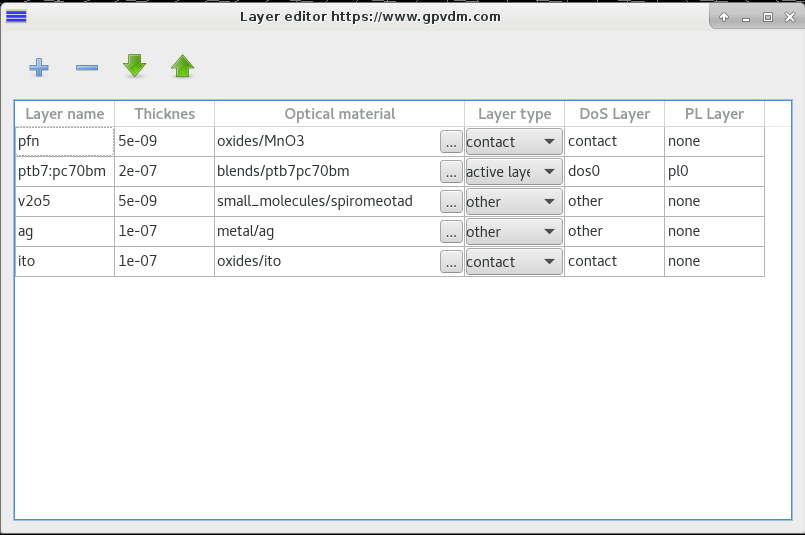
\includegraphics[width=100mm]{./images/layer_editor.png}
{\caption{The contact editor.}}
\label{fig:layer_editor}
\end{figure}

\subsubsection{The contact editor}

The contact editor is used to edit the contacts on the device, and what voltages are applied to which contacts, see figure \ref{fig:contact_editor}.  For a 1D simulation you can pretty much ignore this window.
\linebreak
\linebreak 
\textbf{The first column}: The human readable name for the contact.
\linebreak 
\linebreak 
\textbf{The second column}: Sets if the contact is at the top or bottom of the device.  There should be at least one contact at the top and one contact at the bottom of the device.  Some devices (OFETs) can have more than one contact at the top of the device. 
\linebreak
\linebreak 
\textbf{Third column}: This sets if the contact is 'active'.  In it's simplest form, an active contact is the contact to which the voltage ramp is applied during a JV curve simulation.  In a JV curve simulation, one contact will be held at 0 volts, while a steadily increasing voltage is applied to the other 'active' contact of the device.  If you are performing a transient voltage simulation, such as CELIV, the 'active' contact will have the CELIV voltage transient applied to it.  Swapping around the active contacts is equivalent to picking up the diode and turning it through 180 degrees and placing it back in the circuit.  This feature is most useful, when simulating OFETs, when one wants to apply a voltage ramp to one contact (i.e. the gate) out of three or four.
\linebreak
\linebreak 
\textbf{Forth column}: The start of the contact, not used in 1D simulations
\linebreak
\linebreak 
\textbf{Fifth column}: The width of the contact, not used in 1D simulations.
\linebreak
\linebreak
\textbf{Sixth column}: Sets the pasavation depth under the contact. Not used in 1D simulations.
\linebreak
\linebreak  
\textbf{Seventh column}: The sets the default voltage for a contact.  If the contact type is set as 'active', this value is ignored.  However, it the contact is not active, this voltage will appear on the contact.  This use useful in OFET simulations, where you want to hold a given contact at a set voltage. 
\linebreak
\linebreak  


\begin{figure}[ht!]
\centering
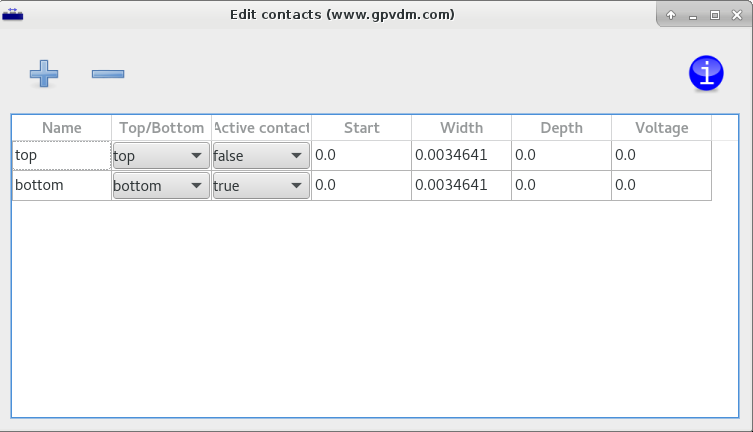
\includegraphics[width=100mm]{./images/contact_editor.png}
{\caption{The contact editor.}}
\label{fig:contact_editor}
\end{figure}



\subsubsection{Scanning parameters}
Sometimes one wishes to systematically vary a simulation parameter, this is how to do it:




\begin{figure}[ht!]
\centering
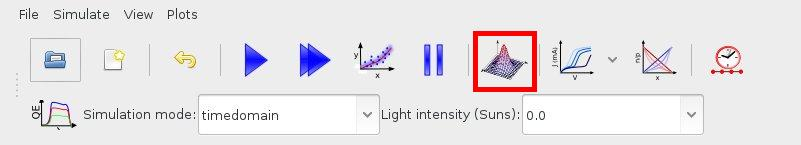
\includegraphics[width=100mm]{./images/1.jpg}
{\caption*{Step 1: Select the 'Parameter scan' tool.}}
\label{overflow}
\end{figure}


\begin{figure}[ht!]
\centering
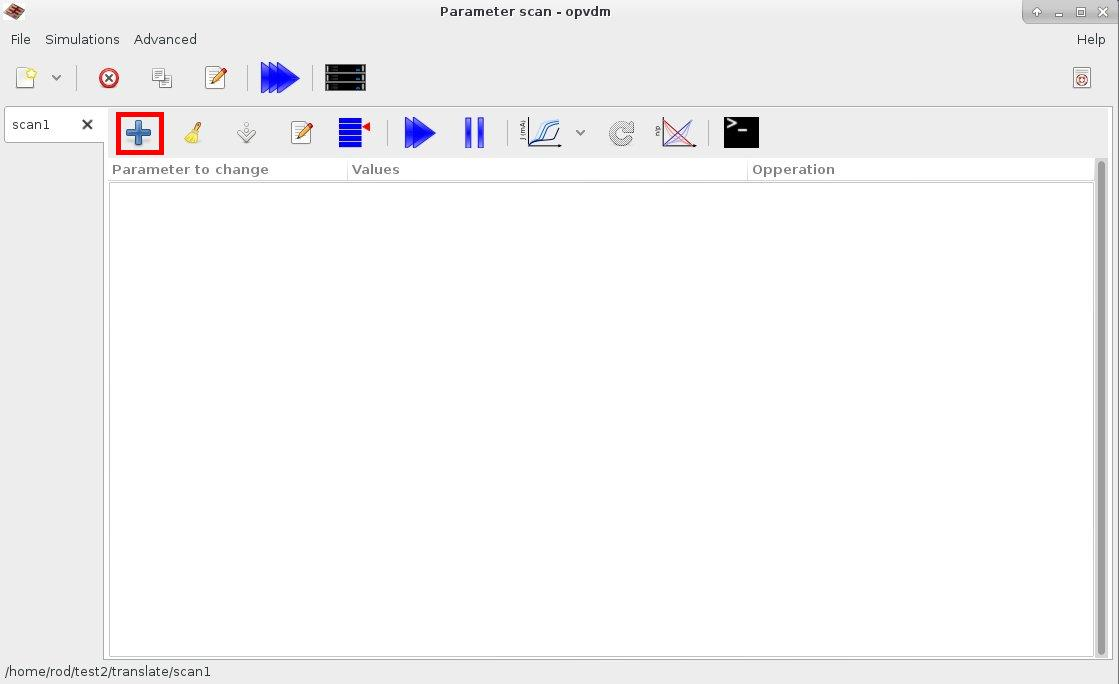
\includegraphics[width=100mm]{./images/2.jpg}
\caption*{Step 2: Add a 'scan line' to the scan.}
\end{figure}

\begin{figure}[ht!]
\centering
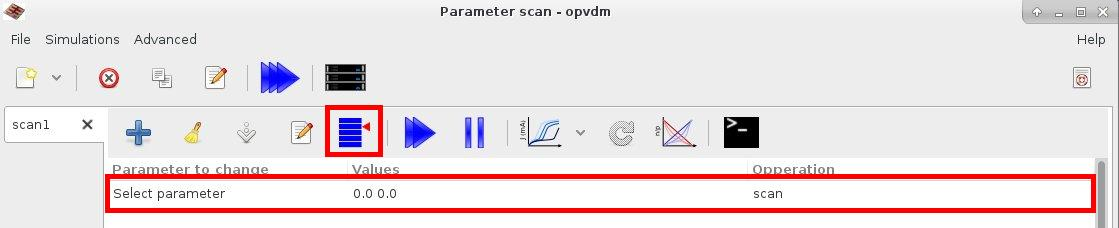
\includegraphics[width=100mm]{./images/3.jpg}
\caption*{Step 3: Select the new 'scan line' and the click on the 'select parameter to change' tool.}
\label{overflow}
\end{figure}


\begin{figure}[ht!]
\centering
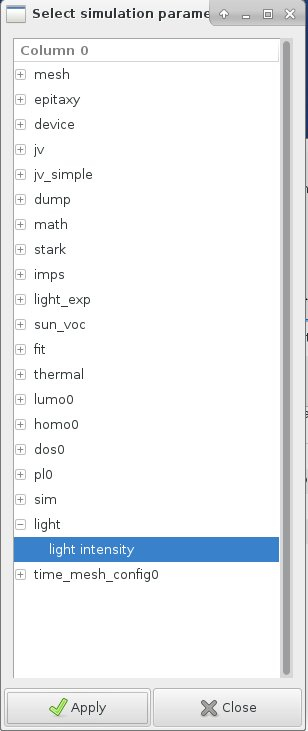
\includegraphics[width=40mm]{./images/4.jpg}
\caption*{Step 4: Select the parameter you want to change, click apply.}
\end{figure}


\begin{figure}[ht!]
\centering
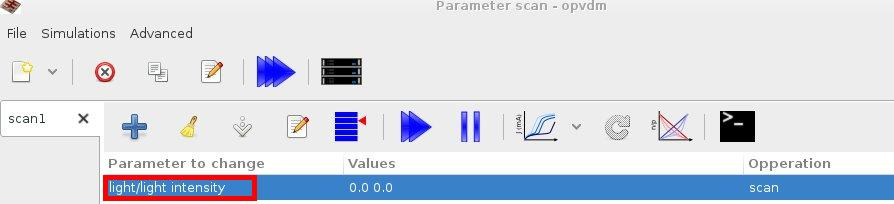
\includegraphics[width=100mm]{./images/5.jpg}
\caption*{Step 5: The 'scan line' should now be updated with the parameter you want to scan.}
\end{figure}


\begin{figure}[ht!]
\centering
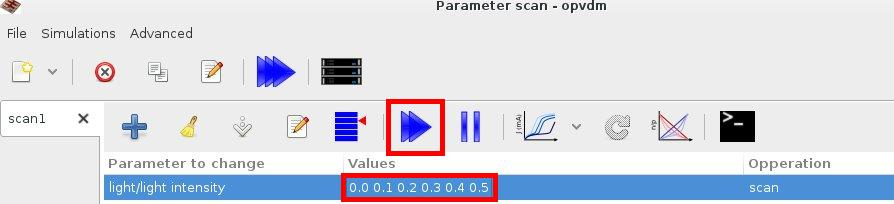
\includegraphics[width=100mm]{./images/6.jpg}
\caption*{Step 6: Now enter the parameters you wish to scan, in this case 0.0-0.5 suns.
Step 7: Click the run button.}
\end{figure}


\begin{figure}[ht!]
\centering
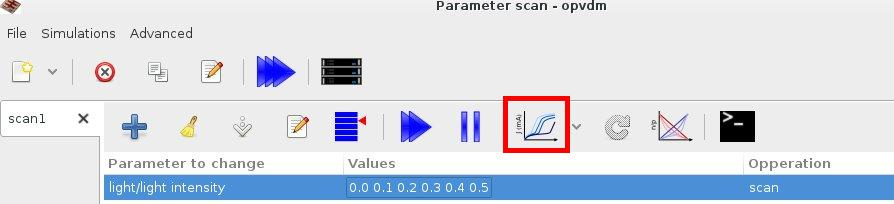
\includegraphics[width=100mm]{./images/7.jpg}
\caption*{Step 8: Select the output file you want to plot.  gpvdm will plot all simulation results.}
\end{figure}

\subsubsection{1D, 2D and 3D simulations with gpvdm}
When deciding if you should perform 1D, 2D or 3D, simulations, consider the dimensionality of your problem.  For example if you consider a solar cell, it is only a few micros thick, and there is rapid variation in the structure, charge densities, mobilities, and doping as a function of depth (y).  However, the structure will not vary very quickly in the lateral (xz) plane.  Therefore, in general  to capture all interesting effects present within a solar cell one only needs a 1D model.  If one now considers OFETs, there is both vertical an lateral current flow, therefore one can not get away with a 1D model any more, as one must simulate both vertical current flow, and current between the source and the drain, thus one needs a 2D simulation.  As the number of dimensions increases, computation speed will decrease, therefore my general advice is to use the minimum number of dimensions possible to solve your problem.

\subsubsection{Why don't I get a 3D view of the device}
If your simulation window looks like figure \ref{fig:nothreed} and not like figure \ref{fig:threed}.  It means  either you do not have any 3D acceleration hardware on your computer, or you do not have the drivers for it installed.  If you have an ATI/Nvidia/Intel graphics card check that the drivers are installed.  Currently, not having working 3D hardware will not affect your ability to perform simulations.

\begin{figure}[ht!]
\centering
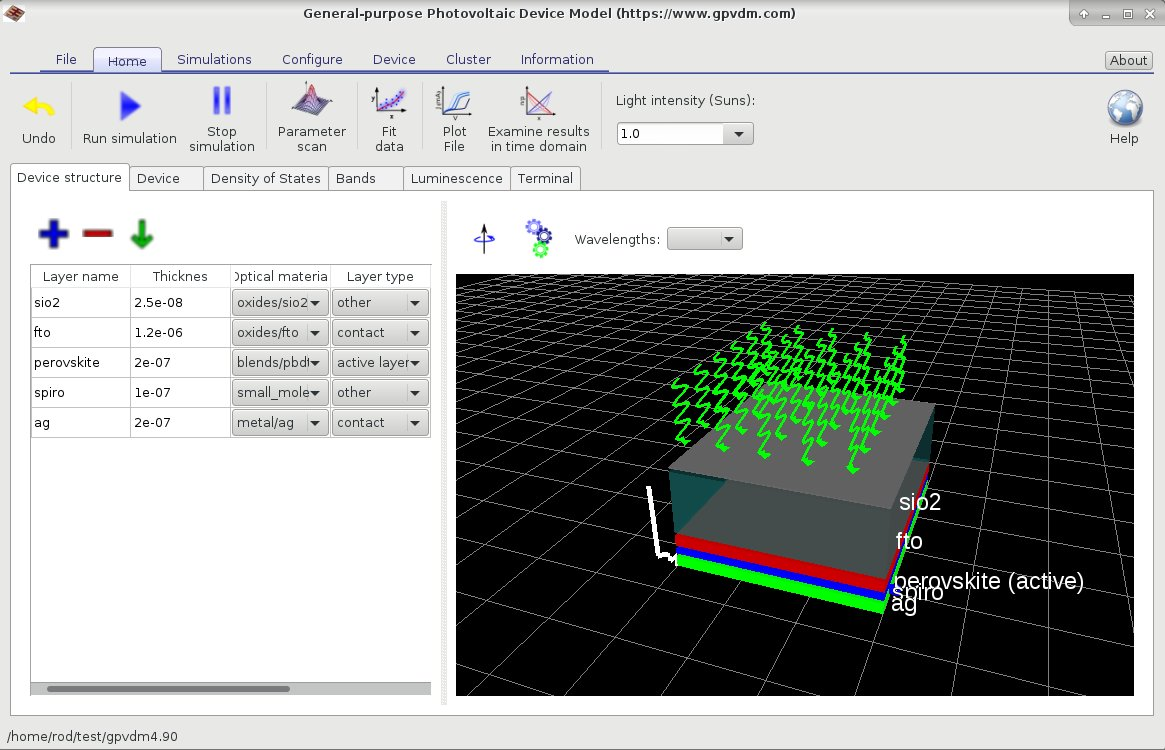
\includegraphics[width=100mm]{./images/3d.jpg}
\caption{gpvdm with working 3D acceleration hardware.}
\label{fig:threed}
\end{figure}

\begin{figure}[ht!]
\centering
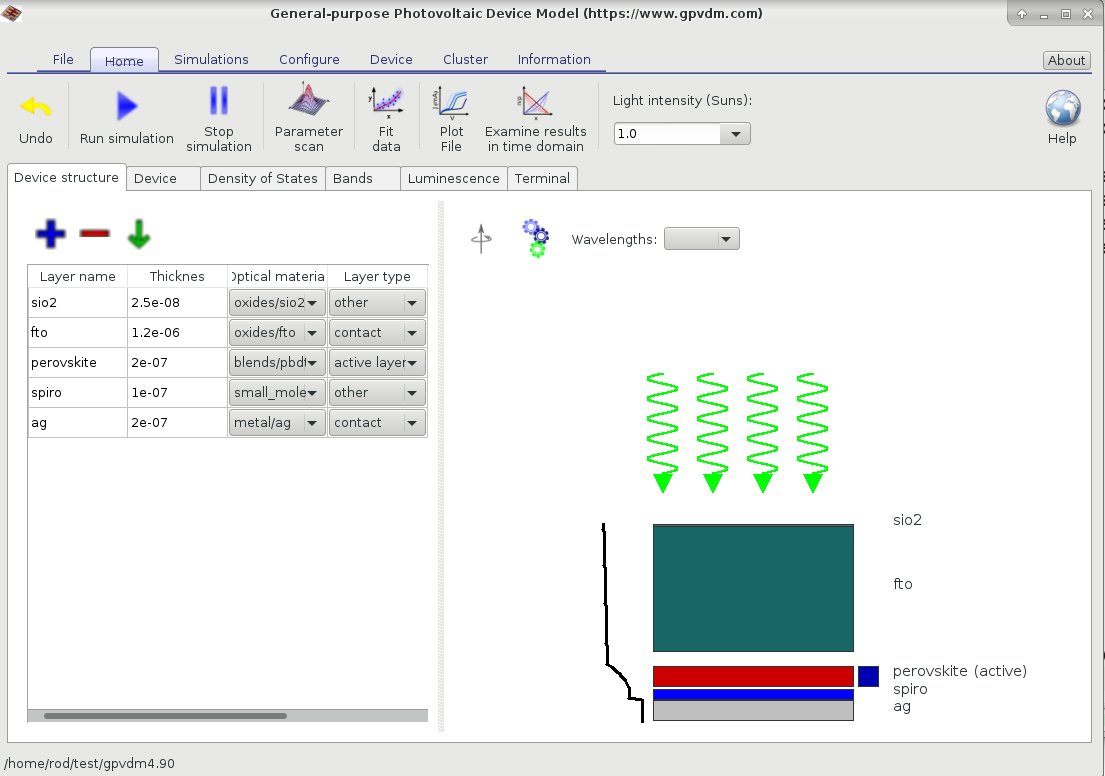
\includegraphics[width=100mm]{./images/no_3d.jpg}
\caption{gpvdm with no 3D acceleration hardware.}
\label{fig:nothreed}
\end{figure}

\vfill
\clearpage

\section{The physical model}
\subsection{Summary of model inputs}
A device is comprised of a series of layers (upto 10 layers), all these layers will interact with light.  Usually only one or two of these layers are electrically active, meaning the transport of electrons and holes must be modeled in detail.  Each electrically active layer with in the device has a set of electrical input parameters which define, charge transport, recombination and trapping. (see table)  If a device has more than one electrically active layer, then multiple sets of these parameters must be defined.  It should be noted that for organic materials (unlike inorganic) there is no standard set of material parameters for any given material.  The exact parameters will depend a lot on the fabrication conditions.  All layers in the device will also need a refractive index spectrum to be defined, this includes the real and imaginary refractive index as a function of wavelength (typically 300-1000 nm).
 
\begin{table}[H]
\begin{center}
\begin{tabular}{lll}
\hline
Parameter & Typical values & unit  \\
\hline
Electron trap density & $0-1.0\e{25}$ & $m^{-3} eV^{-1}$ \\
Hole trap density & $1.0\e{25}$ & $m^{-3} eV^{-1}$ \\
Electron tail slope & $4.0\e{-02}$ & $eV$ \\
Hole tail slope & $4.0\e{-02}$ & $eV$ \\
Electron mobility & $1.0\e{-05}$ & $m^{2}V^{-1}s^{-1}$ \\
Hole mobility & $1.0\e{-05}$ & $m^{2}V^{-1}s^{-1}$ \\
Relative permittivity & $3$ & $au$ \\
Free electron to Trapped electron & $1.0\e{-15}$ & $m^{-2}$ \\
Trapped electron to Free hole & $1.0\e{-28}$ & $m^{-2}$ \\
Trapped hole to Free electron & $1.0\e{-28}$ & $m^{-2}$ \\
Free hole to Trapped hole & $1.0\e{-15}$ & $m^{-2}$ \\
Effective density of free electron states & $5.0\e{+26}$ & $m^{-3}$ \\
Effective density of free hole states & $5.0\e{+26}$ & $m^{-3}$ \\
Xi & $3.7$ & $eV$ \\
Eg & $1.1$ & $eV$ \\
$n_{free}$ to $p_{free}$ Recombination rate constant & $0.0$ & $m^{3}s^{-1}$ \\
  \hline
\end{tabular}
\end{center}
\caption{Device parameters}
\end{table}

\subsection{Summary of model outputs}
The model can output.  Current voltage curves.  The transient responses (current/voltage) to laser pulses, and the response of the the device to the application of a sinusoidal optical or electrical perturbation. 

\subsection{Electrical model}
\subsubsection{Calculating the built in potential}  \label{sssec:initial}
The first step to performing a device simulation, is to calculate the built in potential of the device.  To do this we must know the following things:

\begin{itemize}

  \item The majority carrier concentrations on the contacts $n$ and $p$.
  \item The effective densities of states $N_{LUMO}$ and $N_{HOMO}$.
  \item The effective band gap $E_g$

\end{itemize}

\begin{figure}[ht!]
\centering
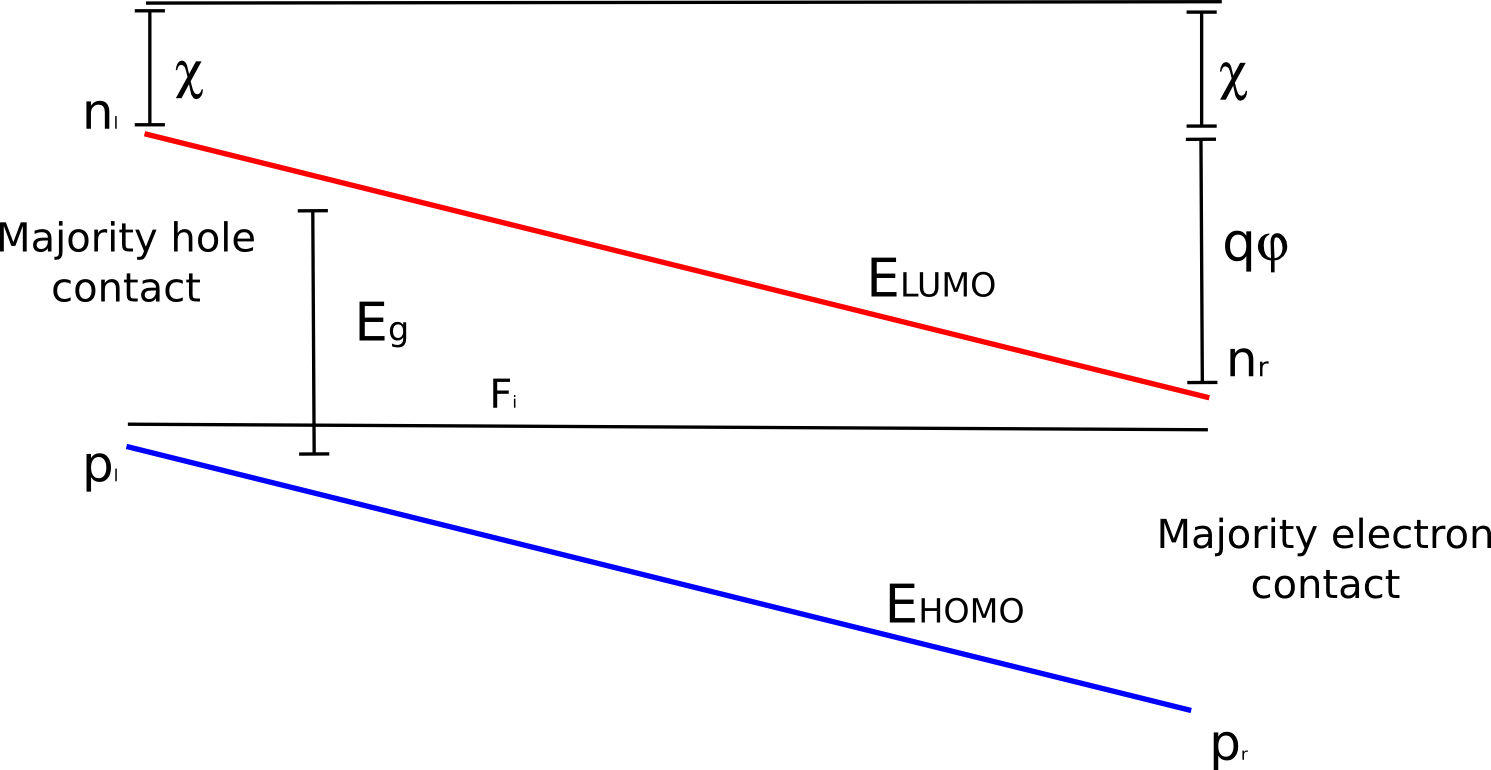
\includegraphics[width=120mm]{./images/bands.png}
\caption{Band structure of device in equilibrium.}
\label{fig:bands}
\end{figure}

\vspace{1em}
The left hand side of the device is given a reference potential of 0 V.  See figure \ref{fig:bands}.  We can then write the energy of the LUMO and HOMO on the left hand side of the device as:

\begin{equation}
E_{LUMO}=-\chi
\end{equation}

\begin{equation}
E_{HOMO}=-\chi-E_{g}
\end{equation}

For the left hand side of the device, we can use Maxwell-Boltzmann statistics to calculate the equilibrium Fermi-level ($F_i$).

\begin{equation}
p_{l}=N_v exp \left(\frac{E_{HOMO}-F_p}{kT} \right)
\end{equation}

We can then calculate the minority carrier concentration on the left hand side using $F_i$

\begin{equation}
n_{l}=N_c exp \left (\frac{F_n-E_{LUMO}}{kT} \right)
\end{equation}

The Fermi-level must be flat across the entire device because it is in equilibrium.  However we know there is a built in potential, we can therefore write the potential of the conduction and valance band on the right hand side of the device in terms of $phi$ to take account of the built in potential.

\begin{equation}
E_{LUMO}=-\chi-q\phi
\label{equ:Ev_rhs}
\end{equation}

\begin{equation}
E_{HOMO}=-\chi-E_g-q\phi
\end{equation}

we can now calculate the potential using

\begin{equation}
n_{r}=N_c exp \left (\frac{F_n-E_{LUMO}}{kT} \right)
\end{equation}
equation \ref{equ:Ev_rhs}.

The minority concentration on the right hand side can now also be calculated using.

\begin{equation}
p_{r}=N_v exp \left (\frac{E_v-F_{HOMO}}{kT} \right)
\end{equation}

The result of this calculation is that we now know the built in potential and minority carrier concentrations on both sides of the device.  Note, infinite recombination velocity on the contacts is assumed.  I have not included finite recombination velocities in the model simply because they would add four more fitting parameters and in my experience I have never needed to use them to fit any experimental data I have come across.

Once this calculation has been performed, we can estimate the potential profile between the left and right hand side of the device, using a linear approximation. From this the charge carrier densities across the device can be guessed.  The guess for potential and carrier densities, is then used to prime the main Newton solver.  Where the real value are calculated.  The Newton solver is described in the next section.

\subsubsection{Transport}
To describe charge carrier transport, the bi-polar drift-diffusion equations are solved in position space
for electrons,
\begin{equation}
\label{eq:ndrive}
\boldsymbol{J_n} = q \mu_e n_{f}  {\frac{\partial E_{LUMO}}{\partial x}}  + q D_n  {\frac{\partial n_{f}}{\partial x}},
\end{equation}
and holes,
\begin{equation}
\label{eq:pdrive}
\boldsymbol{J_p} = q \mu_h p_{f}  {\frac{\partial E_{HOMO}}{\partial x}}  - q D_p {\frac{\partial p_{f}}{\partial x}}.
\end{equation}

Conservation of charge carriers is forced by solving the charge carrier continuity equations for both electrons,
\begin{equation}
\label{eq:contn}
{\frac{\partial \boldsymbol{J_n}}{\partial x}}  = q (R-G),
\end{equation}
and holes
\begin{equation}
\label{eq:contp}
{\frac{\partial \boldsymbol{J_p}}{\partial x}} = - q (R-G).
\end{equation}

where $R$ and $G$ are the net recombination and generation rates per unit volume respectively.

To obtain the internal potential distribution within the device Poisson's equation is solved,

\begin{equation}
\label{eq:pos}
{\frac{d}{d x}} \cdot \epsilon_0 \epsilon_r {\frac{d \phi}{d x}} = q (n_{f}+n_{t}-p_{f}-p_{t}-N_{ad}),
\end{equation}

where $n_{f}$, $n_{t}$ are the carrier densities of free and trapped electrons; $p_{f}$ and $p_{t}$ are the carrier densities of the free and trapped holes; and $N_{ad}$ is the doping density.

\subsubsection{Geminate recombination}
There exist models to calculate the number of charge carriers generated per absorbed photon (and example is the Onsager-Braun model).  This model explicitly accounts for geminate recombination, and charge carrier separation at the microscopic scale.  However, the model will require a number of reliability unknown parameters to make it work, and then as far as solar cell simulation is concerned, you will end up with a number giving you the percentage of absorbed photons which make it to being free electrons/holes.  A more simple approach in my view, is to firstly use correct real/imaginary refractive index spectra for your chosen material.  The optical model will then give you how may photos are absorbed at each position in the device.  Then multiply this generation rate, buy a factor between 0 and 1.0 which accounts for geminate recombination loss.  You can make a good approximation of this value by making sure the simulated and experimental Jsc match up.  This value is set in (Simulation->Optical Simulation->Optical Setup->Photon Efficiency.)


\subsubsection{Carrier trapping and Shockley-Read-Hall recombination}


\begin{figure}
In energy space the model describes the interaction of free carriers with a distribution of trap states using Shockley-Read-Hall (SRH) theory. A 0D section of the model is depicted in figure \ref{fig:dos_structure}, the free electron and hole carrier distributions are labeled as n free and p free respectively. The trapped carrier populations are denoted with n trap and p trap , they are depicted with filled red and blue boxes. SRH theory describes the rates at which electrons and holes become captured and escape from the carrier traps. If one considers a single electron trap, the change in population of this trap can be described by four carrier capture and escape rates as depicted in figure \ref{fig:dos_structure}. The rate rec describes the rate at which electrons become captured into the electron trap, $r_{ee}$ is the rate which electrons can escape from the trap back to the free electron population, $r_{hc}$ is the rate at which free holes get trapped and $r_{he}$ is the rate at which holes escape back to the free hole population. Recombination is described by holes becoming captured into electron space slice through our 1D traps. Analogous processes are also defined for the hole traps.

\centering
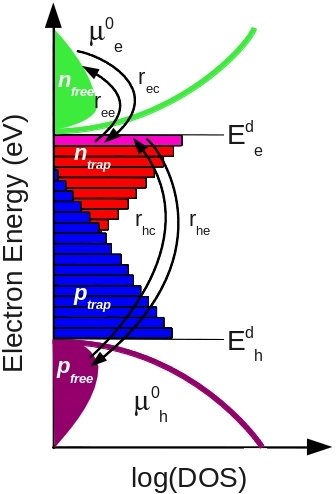
\includegraphics[width=70mm]{./images/dos_structure.jpg}
\caption{Trap filling in both energy and position space as the solar cell is taken from a negative bias
Carrier trapping, de-trapping, and recombination}
\label{fig:dos_structure}
\end{figure}

For each trap level the carrier balance equation

\begin{equation}
\label{eq:taile}
\frac{\delta n_t}{\partial t}=r_{ec}-r_{ee}-r_{hc}+r_{he}
\end{equation}

is solved, giving each trap level an independent quasi-Fermi level. Each point in position space can be allocated between 10 and 160 independent trap states.  The rates of each process $r_{ec}$, $r_{ee}$, $r_{hc}$, and $r_{he}$ are give in table \ref{tab:rates}.

\begin{table}
\begin{center}
  \begin{tabular}{lll}
  \hline
  Mechanism & Label & Description  \\
  \hline
Electron capture rate & $r_{ec}$ & $n v_{th} \sigma_{n} N_{t}(1-f)$ \\
Electron escape rate & $r_{ee}$ & $e_{n} N_{t} f$ \\
Hole capture rate & $r_{hc}$ & $p v_{th} \sigma_{p} N_{t} f$ \\
Hole escape rate & $r_{he}$ & $e_{p} N_{t} (1-f)$\\
  \hline
\end{tabular}
\end{center}
\caption{Shockley-Read-Hall trap capture and emission rates, where $f$ is the fermi-Dirac occupation function and $N_{t}$ is the trap density of a single carrier trap.}
\label{tab:rates}
\end{table}

\begin{equation}
\label{eq:taile}
e_n=v_{th}\sigma_{n} N_{c} exp \left ( \frac{E_t-E_c}{kT}\right )
\end{equation}

and

\begin{equation}
\label{eq:taile}
e_p=v_{th}\sigma_{p} N_{v} exp \left ( \frac{E_v-E_t}{kT}\right )
\end{equation}

 where $\sigma_{n,p}$ are the trap cross sections, $v_{th}$ is the thermal emission velocity of the carriers, and $N_{c,v}$ are the effective density of states for free electrons or holes.  The distribution of trapped states (DoS) is defined between the mobility edges as

\begin{equation}
\label{eq:taile}
\rho^{e/h}(E)=N^{e/h}exp(E/E_{u}^{e/h})
\end{equation}

where , $N_{e/h}$ is the density of trap states at the LUMO or HOMO band edge
in states/eV and where $E_{U}^{e/h}$ is slope energy of the density of states. 

The value of $N_{t}$ for any given trap level is calculated by averaging the DoS function over the energy ($\Delta E$ ) which a trap occupies:

\begin{equation}
\label{eq:taile}
N_{t}(E)=\frac{\int^{E+\Delta E/2}_{E-\Delta E/2} \rho^{e}{E} dE}{\Delta E}
\end{equation}

The ocupation function is given by the equation,
\begin{equation}
f(E_{t},F_{t})=\frac{1}{e^{\frac{E_{t}-F_{t}}{kT}}+1}
\end{equation}
Where, $E_{t}$ is the trap level, and $F_{t}$ is the Fermi-Level of the trap.
The carrier escape rates for electrons and holes are given by


\subsubsection{Free-to-free carrier recombination}
A free-carrier-to-free-carrier recombination pathway is also included in the model. However, most organic solar cells have a great deal of trap states and an ideality factor greater than 1.0 suggesting that free to free recombination is not the dominant mechanism.  It is also worth noting that since I included this recombination pathway in the model I have not found it useful to reproduce experimental results.

Free-to-free recombination is described using equation \ref{equ:freetofree}

\begin{equation}
R_{free}=k_{r}(n_{f}p_{f}-n_{0}-n_{0})
\label{equ:freetofree}
\end{equation}
The above set of non linear equations are placed into a single sparse matrix, and solved using the umfpack solver. The drift diffusion are cast into a Scharfetter-Gummel form, to ensure stability.


\subsection{Discretizing the electrical equations}
Although we assume potential varies linearly between mesh points, the same assumption can not be made for the charge density.  Therefore to ensure numerical stability, the Scharfetter-Gummel approach is used so that the derivative to equation \ref{eq:contn} and \ref{eq:contp} are not evaluated between the left and right mesh point, but at the mid points. To do this we firstly cast the drift diffusion equations as,

\begin{equation}
J_{nx} \rvert_{i+1/2}=n \mu \rvert_{i+1/2} \bigg[ \frac{dE_c}{dx}-\frac{kT}{N_c}\frac{dN_{c}}{dx} \bigg]_{1+1/2}+\mu \rvert_{1+1/2} kT \frac{dn}{dx}
\end{equation}
this is in the form,
\begin{equation}
\frac{dn}{dx}+An=C
\label{eq:ode}
\end{equation}
we can identify the constants as
\begin{equation}
A=\frac{1}{kT}\bigg[ \frac{dE_c}{dx}-\frac{kT}{N_c}\frac{dN_{c}}{dx} \bigg]_{1+1/2}
\end{equation}
and,
\begin{equation}
C=\frac{1}{kT}\frac{J_{nx} \rvert_{i+1/2}}{\mu \rvert_{i+1/2}} .
\end{equation}
Equation \ref{eq:ode} can be written as
\begin{equation}
\frac{d}{dx} \bigg( e^{Ax} n \bigg)=Ce^{Ax}
\end{equation}

which can be integrated between the mesh point $i$ and $i+1$ to give
\begin{equation}
e^{Ax_{i+1}}n_{i+1}-e^{Ax}n_{i}=\frac{C}{A} \bigg( e^{Ax_{i+1}}-e^{Ax} \bigg)
\end{equation}

rearranging gives,
\begin{equation}
=An_{1}\frac{e^{Ax_{i+1}}}{e^{Ax_{i+1}}-e^{Ax_{i}}}-An_{1}\frac{e^{Ax_{i+1}}}{e^{Ax_{i+1}}-e^{Ax_{i}}}
\end{equation}

\begin{equation}
C=\frac{n_{1}}{h_{i+1/2}}\frac{-A h_{i+1/2}}{e^{-Ah_{i+1/2}}-1}-\frac{n_{i+1}}{h_{i+1/2}}\frac{Ah_{i+1/2}}{e^{Ah_{i+1/2}}-1}
\end{equation}

where the definition $h_{i+1/2}=x_{i+1}-x_{i}$ has been used, then using the Bernoulli relation

\begin{equation}
B(x)=\frac{x}{e^{-x}-1}
\end{equation}

one can reformulate the equation as

\begin{equation}
J_{nx} \rvert_{i+1/2} = q \frac{D_{n}\rvert_{i+1/2}}{h_{i+1/2}} \bigg[ B(-\zeta \rvert_{i+1/2}) n_{i+1}- B(\zeta \rvert_{i+1/2}) n_{i} \bigg]
\end{equation}

Care has to be taken to evaluating the Bernoulli expression about zero, so the Taylor expansion is used.  Note, picking the right number of terms has a significant impact on numerical noise in the solver. 

\begin{equation}
B(x)=-\frac{1.0}{2.0}+\frac{x}{6.0}-\frac{x^3}{180}+\frac{x^{5}}{5040}
\end{equation}

The argument to the Bernoulli expression is $\zeta \rvert_{i+1/2}$ is given as

\begin{equation}
\zeta \rvert_{i+1/2}=\frac{h_{i+1/2}}{kT} \bigg( \frac{dE_{c}}{dx}-\frac{kT}{N_c}\frac{dN_{c}}{dx} \bigg) \rvert_{i+1/2}
\end{equation}

A thermal driving term can also be added to the expression, and $N_{c}$ should be reformulated as an effective mass when a temperature gradient is present in the device, due to it's thermal dependence.

\begin{equation}
\zeta \rvert_{i+1/2}=\frac{1}{kT} \Big( E_{c}\rvert_{i+1}-E_{c}\rvert_{i} \Big)-2 \frac{N_{c}\rvert_{i+1}-N_{c}\rvert_{i} }{N_{c}\rvert_{i+1}+N_{c}\rvert_{i} }
\end{equation}

An analogous procedure can be used to derive the the hole current flux which will give

\begin{equation}
J_{p}=q \frac{D_{p}\rvert_{i+1/2}}{h_{i+1/2}} \bigg[ B(-\zeta \rvert_{i+1/2}) p_{i+1}- B(\zeta \rvert_{i+1/2}) p_{i} \bigg]
\end{equation}

\begin{equation}
\zeta_{p} \rvert_{i+1/2}=\frac{1}{kT} \Big( E_{v}\rvert_{i+1}-E_{v}\rvert_{i} \Big)+\frac{N_{v}\rvert_{i+1}-N_{v}\rvert_{i} }{N_{v}\rvert_{i+1}+N_{v}\rvert_{i} }
\end{equation}

The standard finite difference scheme can then be used to rewrite the above equations ready for a computer to solve.


\subsection{Solving the electrical equations}
Key to solving the above equations is picking stable solution variables.  Ideally, the solution variables should minimize the matrix bandwidth to minimize computational overflow and numerical noise.  Through trial and error, the following solution variables were found to be efficient.
\begin{equation}
\zeta_n={q\phi +F_{n}}
\end{equation}

\begin{equation}
\zeta_n=-{q\phi +F_{p}}
\end{equation}

\begin{equation}
\zeta_{nt}={F_{nt}}
\end{equation}

\begin{equation}
\zeta_{pt}={F_{pt}}
\end{equation}

\begin{equation}
\zeta_{Vapplied}=V_{applied}
\end{equation}

The device equations can then be formulated in terms of the above variables, for example the equations linking the Fermi-level to the free carrier concentration can rewritten as

\begin{equation}
n=N_{c}exp(\frac{\zeta_n+\theta_n}{kT})
\end{equation}

\begin{equation}
p=N_{v}exp(\frac{\zeta_p+\theta_p}{kT})
\end{equation}

The band parameters can be defined as

\begin{equation}
\theta_{n}=\frac{\xi}{kT}
\end{equation}

\begin{equation}
\theta_{n}=\frac{\xi+E_{g}}{kT}
\end{equation}

The same can be done with all the SRH capture escape equations.  Once the device equations have been written in terms of the solution variables, they can be reformulated into residual form, in the following way

\begin{equation}
W_{\phi}(\phi,\zeta_{n},\zeta_{p},\zeta_{nt},\zeta_{pt})=0
\end{equation}

\begin{equation}
W_{n}(\phi,\zeta_{n},\zeta_{p},\zeta_{nt},\zeta_{pt})=0
\end{equation}

\begin{equation}
W_{p}(\phi,\zeta_{n},\zeta_{p},\zeta_{nt},\zeta_{pt})=0
\end{equation}

\begin{equation}
W_{nt}(\phi,\zeta_{n},\zeta_{p},\zeta_{nt},\zeta_{pt})=0
\end{equation}

\begin{equation}
W_{pt}(\phi,\zeta_{n},\zeta_{p},\zeta_{nt},\zeta_{pt})=0
\end{equation}

\begin{equation}
W_{i}(\phi,\zeta_{n},\zeta_{p},\zeta_{nt},\zeta_{pt})=0
\end{equation}

We then solve for the corrections to the solution variables, using Newton's method
\begin{equation}
\begin{bmatrix}
\frac{\partial W_{\phi}}{\partial \phi} &
\frac{\partial W_{\phi}}{\partial n} &
\frac{\partial W_{\phi}}{\partial p} &
\frac{\partial W_{\phi}}{\partial nt} &
\frac{\partial W_{\phi}}{\partial pt}\\[0.3em]
\frac{\partial W_{n}}{\partial \phi} &
\frac{\partial W_{n}}{\partial n} &
\frac{\partial W_{n}}{\partial p} &
\frac{\partial W_{n}}{\partial nt} &
\frac{\partial W_{n}}{\partial pt}\\[0.3em]
\frac{\partial W_{p}}{\partial \phi} &
\frac{\partial W_{p}}{\partial n} &
\frac{\partial W_{p}}{\partial p} &
\frac{\partial W_{p}}{\partial nt} &
\frac{\partial W_{p}}{\partial pt}\\[0.3em]
\frac{\partial W_{nt}}{\partial \phi} &
\frac{\partial W_{nt}}{\partial n} &
\frac{\partial W_{nt}}{\partial p} &
\frac{\partial W_{nt}}{\partial nt} &
\frac{\partial W_{nt}}{\partial pt}\\[0.3em]
\frac{\partial W_{pt}}{\partial \phi} &
\frac{\partial W_{pt}}{\partial n} &
\frac{\partial W_{pt}}{\partial p} &
\frac{\partial W_{pt}}{\partial nt} &
\frac{\partial W_{pt}}{\partial pt}\\[0.3em]
\end{bmatrix}
\begin{bmatrix}
\Delta \zeta_\phi \\[0.3em]
\Delta \zeta_{n}\ \\[0.3em]
\Delta \zeta_{p}\ \\[0.3em]
\Delta \zeta_{nt}\ \\[0.3em]
\Delta \zeta_{pt}\ \\[0.3em]
\end{bmatrix}
=-
\begin{bmatrix}
W_\phi \\[0.3em]
W_{n}\ \\[0.3em]
W_{p}\ \\[0.3em]
W_{nt}\ \\[0.3em]
W_{pt}\ \\[0.3em]
\end{bmatrix}
\end{equation}

The boundary conditions used in solving this system of differential equations are taken as the electron/hole densities on either side of the device, and the built in potential as calculated in  \ref{sssec:initial}.  To move from a equilibrium conditions to a state where current is flowing the potential either side of the device is updated so that the system is no longer in equilibrium.  The system of equations is then resolved, and current will be flowing.

\subsubsection{Numerical clamping}
Newton's method will always give an update vector in the direction of the solution.  However, often the update vector is non-optimal for convergence.  Very often the update is too large and will jump over the solution, leading the solver far away from the desired answer.  More often than not if this happens the solver will crash, as it will find it's self in an unphysical space.  There have been many method proposed, to help Newton's take an optimal step towards the solution.  Once is back tracking (see numerical recipes in C) which in general has a computational overhead to implement, and another faster possibility is numerical clamping.  In gpvdm, we use clamping, updates to the solution variables are clamped by the following scheme.

\begin{equation}
\Delta \zeta_n=\frac{\Delta \zeta_n}{1.0+|\frac{q \Delta \zeta_n}{c300\kappa}|}
\end{equation}

\begin{equation}
\Delta \zeta_{\phi}=\frac{\Delta \zeta_{\phi}}{1.0+|\frac{q \Delta \zeta_{\phi}}{c300\kappa}|}
\end{equation}

\begin{equation}
\Delta \zeta_{n}=\frac{\Delta \zeta_{n}}{1.0+|\frac{q \Delta \zeta_{n}}{c300\kappa}|}
\end{equation}

\begin{equation}
\Delta \zeta_{p}=\frac{\Delta \zeta_{p}}{1.0+|\frac{q \Delta \zeta_{p}}{c300\kappa}|}
\end{equation}

\begin{equation}
\Delta \zeta_{nt}=\frac{\Delta \zeta_{nt}}{1.0+|\frac{q \Delta \zeta_{nt}}{c300\kappa}|}
\end{equation}

\begin{equation}
\Delta \zeta_{pt}=\frac{\Delta \zeta_{pt}}{1.0+|\frac{q \Delta \zeta_{pt}}{c300\kappa}|}
\end{equation}

The variable $c$ is defined in the math.inp input file.

\subsubsection{External circuit elements}
The above equations will simply solve the diode equation for an ideal diode.  They neglect, the parasitic components of the diode, namely the shunt resistance, the series resistance and the parasitic capacitance.   For simulating a JV curve, it is a simple matter to convert from the ideal diode voltage/current curve to the non ideal curve.  One simply performs a JV curve sweep for an ideal diode, then uses the following equations to generate the non-ideal JV curve, including parasitic components.

\begin{equation}
j_{external}=i_{ideal}+\frac{V_{applied}}{R_{shunt}}
\end{equation}

where $i(V_{applied})$, is calculated from the current at the contacts $(j_{left}+j_{right})/2$.

\begin{equation}
V_{external}=V_{ideal}+R_{series}j_{external}
\end{equation}

This is an efficient procedure.  For some measurements however, such as transient photovoltage, the situation becomes more complex, as one has to find $V_{applied}$, to suite the desired conditions.  For example when finding $V_{oc}$ (or indeed performing a TPV simulation), one is looking for the value of $V_{applied}$, which will give $j_{external}=0$.  Clearly one way to do this would be to search a reasonable range of $V_{applied}$ until the condition $j_{external}=0$ is met.  This would however be slow, especially if one is having to repeat the procedure multiple times, such as in a time domain simulation.  A better method is to first guess the value of $V_{applied}$ which could cause the condition $j_{external}=0$ to be met (a good guess may be the value of the built in bias), then to iterate using an external newton solver, to update $V_{applied}$ until the condition $j_{external}=0$, is met to the desired degree of accuracy.  This is more efficient than a linear search for $V_{oc}$, however it is still inefficient, as it will require two Newton solvers, one for the diode equations (described above) and one to enforce $j_{external}=0$.  When one couples together two Newton solvers, convergence is not guaranteed, in fact they can oscillate and diverge.  Also, convergence will probably proceed in a linear fashion, rather than a super-linear fashion.  The equations to external circuits, in an external newton solver is included in gpvdm as an option, mainly for debugging.  Another difficulty with simulating TPV, is the precision one can solve the diode current to is of the order of $1\e-6$-$1\e-7$ Amps, and a typical value of shunt resistance is around $1\e6$ Ohms, this the numerical noise in the solver can very easily be amplified by the shunt resistance to a level where the whole system of equations becomes unstable.  Solving, the system of equations in a coupled form expatiates this problem.

A better way to solve for the presence of external circuit elements is to, include another solution variable in the main Newton solver, namely $V_{applied}$.  This avoids the need of two coupled solvers.  This is a single value of potential, which defines the applied voltage to the device. The updated solution matrix will look like this

\begin{equation}
\begin{bmatrix}
\frac{\partial W_{\phi}}{\partial \phi} &
\frac{\partial W_{\phi}}{\partial n} &
\frac{\partial W_{\phi}}{\partial p} &
\frac{\partial W_{\phi}}{\partial nt} &
\frac{\partial W_{\phi}}{\partial pt} &
\frac{\partial W_{\phi}}{\partial V_{applied}} \\[0.3em]
\frac{\partial W_{n}}{\partial \phi} &
\frac{\partial W_{n}}{\partial n} &
\frac{\partial W_{n}}{\partial p} &
\frac{\partial W_{n}}{\partial nt} &
\frac{\partial W_{n}}{\partial pt} &
\frac{\partial W_{n}}{\partial V_{applied}} \\[0.3em]
\frac{\partial W_{p}}{\partial \phi} &
\frac{\partial W_{p}}{\partial n} &
\frac{\partial W_{p}}{\partial p} &
\frac{\partial W_{p}}{\partial nt} &
\frac{\partial W_{p}}{\partial pt} &
\frac{\partial W_{p}}{\partial V_{applied}} \\[0.3em]
\frac{\partial W_{nt}}{\partial \phi} &
\frac{\partial W_{nt}}{\partial n} &
\frac{\partial W_{nt}}{\partial p} &
\frac{\partial W_{nt}}{\partial nt} &
\frac{\partial W_{nt}}{\partial pt} &
\frac{\partial W_{nt}}{\partial V_{applied}} \\[0.3em]
\frac{\partial W_{pt}}{\partial \phi} &
\frac{\partial W_{pt}}{\partial n} &
\frac{\partial W_{pt}}{\partial p} &
\frac{\partial W_{pt}}{\partial nt} &
\frac{\partial W_{pt}}{\partial pt} &
\frac{\partial W_{pt}}{\partial V_{applied}} \\[0.3em]
\frac{\partial W_{V_{applied}}}{\partial \phi} &
\frac{\partial W_{V_{applied}}}{\partial n} &
\frac{\partial W_{V_{applied}}}{\partial p} &
\frac{\partial W_{V_{applied}}}{\partial nt} &
\frac{\partial W_{V_{applied}}}{\partial pt} &
\frac{\partial W_{V_{applied}}}{\partial V_{applied}} \\[0.3em]
\end{bmatrix}
\begin{bmatrix}
\Delta \zeta_\phi \\[0.3em]
\Delta \zeta_{n}\ \\[0.3em]
\Delta \zeta_{p}\ \\[0.3em]
\Delta \zeta_{nt}\ \\[0.3em]
\Delta \zeta_{pt}\ \\[0.3em]
\Delta \zeta_{V_{applied}}\ \\[0.3em]
\end{bmatrix}
\\
=-
\begin{bmatrix}
W_\phi \\[0.3em]
W_{n}\ \\[0.3em]
W_{p}\ \\[0.3em]
W_{nt}\ \\[0.3em]
W_{pt}\ \\[0.3em]
W_{V_{applied}}\ \\[0.3em]
\end{bmatrix}
\end{equation}

Note, the derivatives of $W_{\phi}$,$W_{n}$,$W_{p}$,$W_{nt}$,$W_{pt}$, which are functions of $V_{applied}$, now also have to be calculated.  In practice, only the far right hand (or left) of the finite difference grid next to the contacts will be non zero.  Now, to solve any external circuit under any desired condition, one simply has to couch the equation describing the external circuit in the form of a residual equation,
\begin{equation}
W_{V_{applied}}(\phi,\zeta_{n},\zeta_{p},\zeta_{nt},\zeta_{pt},V_{applied})=0 .
\end{equation}

For example, in the most simple case, if one wants to solve for a given internal diode voltage, one can write 

\begin{equation}
W_{V_{applied}}(\phi,\zeta_{n},\zeta_{p},\zeta_{nt},\zeta_{pt},V_{applied})=V_{applied}-V_{desired}
\end{equation}

in this case,

\begin{equation}
\frac{\partial W_{V_{applied}}}{\partial V_{applied}}=1.0
\end{equation}

where $V_{desired}$, is the desired output voltage. Or for another example, if one wants to solve for $V_{oc}$ one can write

\begin{equation}
W_{V_{applied}}(\phi,\zeta_{n},\zeta_{p},\zeta_{nt},\zeta_{pt},V_{applied})=V_{applied}-i(V_{applied})*R_{shunt}
\end{equation}

which forces the current going through the shunt resistance to equal that the diode is generating.  Appropriate, derivatives of $W_{V_{applied}}(\phi,\zeta_{n},\zeta_{p},\zeta_{nt},\zeta_{pt},V_{applied})$, would then have to be calculated.

\subsubsection{Average free carrier mobility}
In this model there are two types of electrons (holes), free electrons (holes) and trapped electrons (holes).  Free electrons (holes) have a finite mobility of $\mu_e^0$ ($\mu_h^0$) and trapped electrons (holes) can not move at all and have a mobility of zero.  To calculate the average mobility we take the ratio of free to trapped carriers and multiply it by the free carrier mobility.:

\begin{equation}
\mu_e(n)=\frac{\mu_e^0 n_{free}}{n_{free}+n_{trap}}
\end{equation}

Thus if all carriers were free, the average mobility would be $\mu_e^0$ and if all carriers were trapped the average mobility would be 0.  It should be noted that only $\mu_e^0$ ($\mu_h^0$) are used in the model for computation and $\mu_e(n)$ is an output parameter.

The value of $\mu_e^0$ ($\mu_h^0$) is an input parameter to the model.  This can be edited in the electrical parameter editor.  The value of $\mu_e(n)$, and $\mu_h(p)$ are output parameters from the model.  The value of $\mu_e(n)$, and $\mu_h(p)$ change as a function of position, within the device, as the number of both free and trapped charge carriers change as a function of position.  The values of  $\mu_e(x)$, and $\mu_h(x)$ can be found in $mu\_n\_ft.dat$ and $mu\_p\_ft.dat$ within the $snapshots$ directory.  The spatially averaged value of mobility, as a function of time or voltage can be found in the files $dynamic\_mue.dat$ or $dynamic\_muh.dat$ within the dynamic directory.

Were one to try to measure mobility using a technique such as CELIV or ToF, one would expect to get a value closer to $\mu_e(n)$ or $\mu_h(p)$ rather than closer to $\mu_e^0$ or $\mu_h^0$.  It should be noted however, that measuring mobility in disordered materials is a difficult thing to do, and one will get a different experimental value of mobility depending upon which experimental measurement method one uses, furthermore, mobility will change depending upon the charge density profile within the device, and thus upon the applied voltage and light intensity.  To better understand this, try for example doing a CELIV simulation, and plotting $\mu_e(n)$ as a function of time (Voltage).  You will see that mobility reduces as the negative voltage ramp is applied, this is because carriers are being sucked out of the device.  Then try extracting the mobility from the transient using the CELIV equation for extracting mobility.  Firstly, the CELIV equation will give you one value of mobility, which is a simplification of reality as the value really changes during the application of the voltage ramp.  Secondly, the value you get from the equation will almost certainly not match either $\mu_e^0$ or any value of $\mu_e(n)$.  This simply highlights, the difficult of measuring $a$ value of mobility for a disordered semiconductor and that really when we quote a value of mobility for a disordered material, it really only makes sense to quote a value measured under the conditions a material will be used.  For example, for a solar cell, values of $\mu_e(n)$ and $\mu_h(n)$, would be most useful to know under 1 Sun at the $P_{max}$ point on a JV curve.

\subsubsection{Energy balance - hydrodynamic transport model}
This is an experimental feature.  From the configure window one can access the thermal simulation tab \ref{fig:thermal}, by default this model is turned off.  There are three options, the lattice thermal model which just solves the lattice heat equation; electron thermal model and hole thermal model.  The latter two solve the energy balance equations, or 3rd order moment expansion of of the Boltzmann equation.  If you turn on just the lattice model, the lattice heat equation will be solved along with the electrical model.  The thermal solver is external to the electrical solver. 

\begin{equation}
 \frac{d}{dx}\Bigg(-  \kappa_{l} \frac{dT_{L}}{dt}\Bigg)=H
\end{equation}
where H (the heat source term) is given by

\begin{equation}
H=\frac{1}{q}\frac{dE_{c}}{dx} J_{n}+\frac{1}{q}\frac{dE_{v}}{dx} J_{p}+R(E_{c}-E_{v})
\end{equation}

If you turn on the electrical and hole thermal model, then the heat source term will be replaced by

\begin{equation}
H=\frac{3 k_{b}}{2} \Bigg ( n (\frac{T_{n}-T_{l}}{\tau_{e}}) + p (\frac{T_{p}-T_{l}}{\tau_{h}})\Bigg) +R(E_{c}-E_{v})
\end{equation}

and the energy transport equation for electrons

\begin{equation}
S_n=-\kappa_n \frac{dT_{n}}{dx}-\frac{5}{2} \frac{k_{b}T_{n}}{q} J_{n}
\end{equation}

and holes,

\begin{equation}
S_p=-\kappa_p \frac{dT_{p}}{dx}+\frac{5}{2} \frac{k_{b}T_{p}}{q} J_{p}
\end{equation}

will be solved.

The energy balance equations will also be solved for electrons,

\begin{equation}
\frac{dS_{n}}{dx}=\frac{1}{q}\frac{dE_{c}}{dx} J_{n}-\frac{3 k_{b}}{2} \Bigg( R T_{n}+ n(\frac{T_{n}-T_{l}}{\tau_{e}}) \Bigg)
\end{equation}

and for holes

\begin{equation}
\frac{dS_{p}}{dx}=\frac{1}{q}\frac{dE_{v}}{dx} J_{p}-\frac{3 k_{b}}{2} \Bigg( R T_{p}+ n(\frac{T_{p}-T_{l}}{\tau_{e}}) \Bigg)
\end{equation}

The thermal conductivity of the electron gas is given by

\begin{equation}
\kappa_{n}=\Bigg ( \frac{5}{2} +c_n\Bigg) \frac{{k_{b}}^2}{q} T_{n} \mu_n n
\end{equation}

and for holes as,

\begin{equation}
\kappa_{p}=\Bigg ( \frac{5}{2} +c_p\Bigg) \frac{{k_{b}}^2}{q} T_{p} \mu_p p
\end{equation}


\begin{figure}[!htb]
\centering
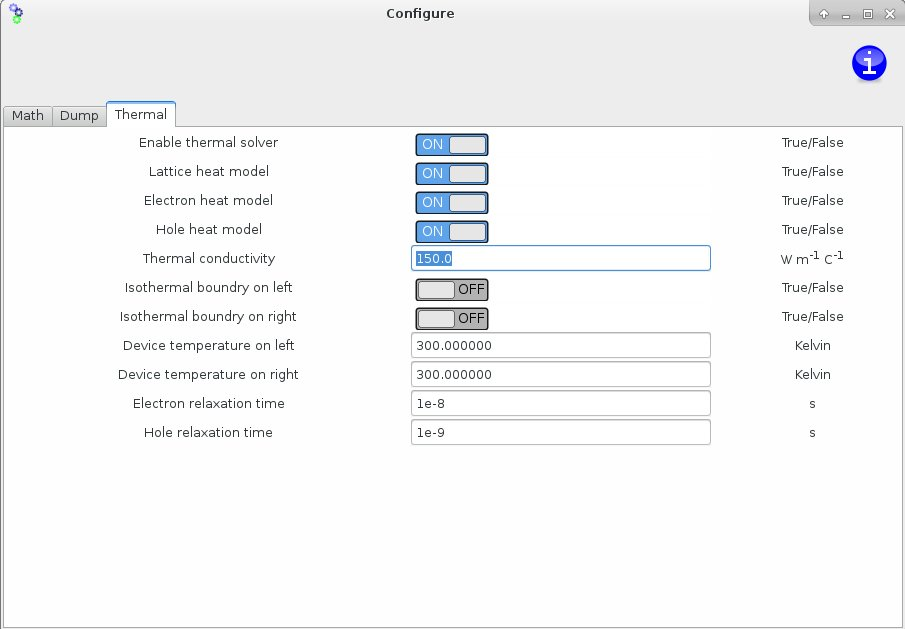
\includegraphics[width=100mm]{./images/thermal.jpg}
{\caption{The thermal configuration window}}
\label{fig:thermal}
\end{figure}

\subsection{Optical model}
On the left of the interface the electric field is given by
\begin{equation}
E_{1}=E^{+}_{1} e^{-j k_1 z}+E^{-}_{1} e^{j k_1 z}
\label{efield1}
\end{equation}
and on the right hand side of the interface the electric field is given by
\begin{equation}
E_{2}=E^{+}_{2} e^{-j k_2 z}+E^{-}_{2} e^{j k_2 z}
\label{efield2}
\end{equation}

Maxwel's equations give us the relationship between the electric and magnetic fields for a plane wave.

\begin{equation}
\nabla \times E=-j\omega \mu H 
\end{equation}
which simplifies to:
\begin{equation}
\frac{\partial E} {\partial z}=-j\omega \mu H 
\label{maxwel}
\end{equation}

Applying equation \ref{maxwel} to equations \ref{efield1}-\ref{efield2}, we can get the magnetic field on the left of the interface
\begin{equation}
-j \mu \omega H^{y}_{1}=-j k_1 E^{+}_{1} e^{-j k_1 z}+j k_1 E^{-}_{1} e^{j k_1 z}
\end{equation}
and on the right of the interface
\begin{equation}
-j \mu \omega H^{y}_{2}=-j k_2 E^{+}_{2} e^{-j k_2 z}+j k_2 E^{-}_{2} e^{j k_2 z}.
\end{equation}

Tidying up gives,
\begin{equation}
H^{y}_{1}=\frac{k}{\omega \mu}E^{+}_{1} e^{-j k_1 z}-\frac{k}{\omega \mu} E^{-}_{1} e^{j k_1 z}
\end{equation}

\begin{equation}
H^{y}_{2}=\frac{k}{\omega \mu}E^{+}_{2} e^{-j k_2 z}-\frac{k}{\omega \mu} E^{-}_{2} e^{j k_2 z}
\end{equation}

\subsubsection{Boundary conditions}
We now apply the electric and magnetic boundary conditions\cite{0953-8984-25-21-215301}
\begin{equation}
\mathbf{n} \times (\mathbf{E_2}-\mathbf{E_1})=0
\end{equation}

\begin{equation}
\mathbf{n} \times (\mathbf{H_2}-\mathbf{H_1})=0
\end{equation}

We let the interface be at z=0, which gives,
\begin{equation}
(E_{2}^{+}+E_{2}^{-})-(E_{1}^{+}+E_{1}^{-})=0
\label{electric_boundary}
\end{equation}
and
\begin{equation}
\frac{k_1}{\omega \mu}(E_{2}^{+}-E_{2}^{-})-(E_{1}^{+}-E_{1}^{-})\frac{k_2}{\omega \mu}=0
\end{equation}
.
The wavevector is given by
\begin{equation}
k=\frac{2 \omega }{\lambda}=\frac{\omega n}{c}
\end{equation}
.
We can therefore write the magnetic boundary condition as
\begin{equation}
n_2 (E_{2}^{+}-E_{2}^{-}) - n_1 (E_{1}^{+}-E_{1}^{-})=0
\label{mag_boundary}
\end{equation}

\subsubsection{Forward propagating wave}
Rearrange equation, \ref{mag_boundary} to give,

\begin{equation}
E_{1}^{-} = E_{1}^{+}-\frac{n_2}{n_1}(E_{2}^{+}-E_{2}^{-})
\end{equation}
Inserting in equation \ref{electric_boundary}, gives 
\begin{equation}
E_{2}^{+}+E_{2}^{-}=E_{1}^{+}+E_{1}^{+}-\frac{n_2}{n_1}(E_{2}^{+}-E_{2}^{-})
\end{equation}

\begin{equation}
2E_{1}^{+}=E_{2}^{+}+E_{2}^{-}+\frac{n_2}{n_1}(E_{2}^{+}-E_{2}^{-})
\end{equation}

\begin{equation}
2E_{1}^{+}\frac{n_1}{n_1+n_2}=E_{2}^{+}+E_{2}^{-}\frac{n_1-n_2}{n_1+n_2}
\end{equation}

\subsubsection{Backwards propagating wave}
Rearrange equation, \ref{mag_boundary} to give,

\begin{equation}
E_{1}^{+}=E_{1}^{-} +\frac{n_2}{n_1}(E_{2}^{+}-E_{2}^{-})
\end{equation}

Inserting in equation \ref{electric_boundary}, gives 
\begin{equation}
E_{2}^{+}+E_{2}^{-}=E_{1}^{-} +\frac{n_2}{n_1}(E_{2}^{+}-E_{2}^{-})+E_{1}^{-}
\end{equation}

\begin{equation}
2E_{1}^{-}=E_{2}^{+}+E_{2}^{-}- \frac{n_2}{n_1}(E_{2}^{+}-E_{2}^{-})
\end{equation}

\begin{equation}
2E_{1}^{-}\frac{n_1}{n_1+n_2}=E_{2}^{+}\frac{n_1-n_2}{n_1+n_2}+E_{2}^{-}
\end{equation}
Which is the same result as obtained in \cite{10.1063/1.1534621}.

These equations become:

\begin{equation}
E_{1}^{-}t_{12}=E_{2}^{+}r_{12}+E_{2}^{-}
\end{equation}

and
\begin{equation}
E_{1}^{+}t_{12}=E_{2}^{+}+E_{2}^{-}r_{12}
\end{equation}

Accounting for propagation we can write.  Note the change in sign between \cite{10.1063/1.1534621} and this work, this is because of how I have defined my wave equation. 
\begin{equation}
E_{1}^{+}t_{12}=E_{2}^{+}e^{\zeta_2 d_1}+E_{2}^{-}r_{12}e^{-\zeta_2 d_1}
\end{equation}
and

\begin{equation}
E_{1}^{-}t_{12}=E_{2}^{+}r_{12}e^{\zeta_2 d_1}+E_{2}^{-}e^{-\zeta_2 d_1}
\end{equation}

where
\begin{equation}
\zeta=\frac{2\pi}{\lambda} \bar{n}
\end{equation}

Note that in  \cite{10.1063/1.1534621} they use $\zeta_1$ instead of $\zeta_2$.  This is a mistake and makes a difference at interfaces.
For a device with non reflecting back contacts:

$
 \begin{pmatrix}
  e^{\zeta d}         & 0                   & 0                  & 0                   &r_{01}e^{-\zeta d}     & 0                       & 0                    & 0   \\
  -t_{12}              & e^{\zeta d}        & 0                  & 0                   &0                     & r_{12}e^{-\zeta d}      & 0                   & 0    \\
  0                    & -t_{23}             & e^{\zeta d}       & 0			&0                     & 0                      & r_{23}e^{-\zeta d}   & 0    \\
  0                    & 0                   & -t_{34}            & e^{\zeta d}	& 0			& 0                      & 0                   & r_{34}e^{-\zeta d} \\
  0                    &r_{12}e^{\zeta d_1} & 0                   & 0                  & -t_{12}			&e^{-\zeta d}           & 0                      & 0       \\
  0                    &0                    & r_{23}e^{\zeta d}  & 0                  & 0                     	   &-t_{23}                & e^{-\zeta d}           & 0    \\
  0                    &0                    & 0                   & r_{34}e^{\zeta d} & 0     			   &0                     & -t_{34}                & e^{-\zeta d}    \\
  0                    &0                    & 0                   & 0		  	& 0				   &0                     & 0			   & -t_{45}        \\
 \end{pmatrix}
\begin{pmatrix}
  E_{1}^{+} \\
  E_{2}^{+} \\
  E_{3}^{+}  \\
  E_{4}^{+} \\
  E_{1}^{-} \\
  E_{2}^{-} \\
  E_{3}^{-}  \\
  E_{4}^{-}  \\
 \end{pmatrix}
=
\begin{pmatrix}
  t_{01}E_{external} \\
  0 \\
  0 \\
  0 \\
  0 \\
  0 
 \end{pmatrix}
$



The boundary condition on the right hand side is given by:
\begin{equation}
E_{4}^{-}t_{45}=E_{5}^{+}r_{45}e^{\zeta_1 d_1}+E_{5}^{-}e^{-\zeta_1 d_1}
\end{equation}
where we say that $E_{5}^{-}$ is zero and $r_{12}$ is zero.  Therefore we end up with

\begin{equation}
E_{4}^{-}t_{45}=0
\end{equation}
as the boundary condition.

\subsubsection{Refractive index and absorption}
\begin{equation}
E(z,t)=Re(E_0 e^{j(-kz+\omega t)})= Re(E_0 e^{j(\frac{-2 \pi (n+j\kappa)}{\lambda}z + \omega t)})=e^{\frac{2\pi\kappa z}{\lambda}}Re(E_0 e^{\frac{j(-2 \pi (n+j\kappa)}{\lambda}z +\omega t})
\end{equation}
And because the intensity is proportional to the square of the electric field the absorption coefficient becomes

\begin{equation}
e^{-\alpha x}=e^{\frac{2\pi\kappa z}{\lambda}}
\end{equation}

\begin{equation}
\alpha=-\frac{4\pi\kappa}{\lambda_0}
\end{equation}

\subsubsection{Why has the efficency of my solar cell changed now that I have upgraded to gpvdm v 4.97+}
My self and my students have recently put a lot of effort into improving the materials data base.  This means improved, absorption and refractive index data, this can affect the calculate device efficiency.  If you want to reproduce a device efficiency from a previous version of gpvdm, go to Simulations->Optica Simulation->Optical setup->Photon Efficiency. And play with this value, until you can reproduce the old efficiency.  You should only have to change the value by 20\% or so.

\subsubsection{Is Langevin recombination a good way of describing recombination OPV devices?}
In my view Langevin recombination is in general a really bad way to describe recombination in OPV devices.  This is because the mechanism assumes Brownian motion of electrons and holes and that charge carriers of opposite polarity will recombine when they get close enough to fall into each others electrostatic field.  This picture assumes the charge carriers are free and completely neglects the influence of trap states.  I therefore think Langeving recombination should be avoided in OPVs.
But in dx.doi.org/10.1021/jp200234m you used Langevin recombination - why?: In this paper I allowed the mobility in the Langevin expression to vary as a function of carrier density i.e.
\begin{equation}
R_{free}=q k_{r}\frac{(\alpha \mu_e(n)+\beta \mu_h(n)) n_{tot} p_{tot}}{2\epsilon_0\epsilon_r}
\end{equation}

I then by defining a mobility edge and assuming any carrier below the mobility edge could not move and any carrier above it could.  I could define the averaged electron/hole mobility as: 

\begin{equation}
\mu_e(n)=\frac{\mu_e^0 n_{free}}{n_{free}+n_{trap}}
\end{equation}

and

\begin{equation}
\mu_h(n)=\frac{\mu_h^0 p_{free}}{p_{free}+p_{trap}}
\end{equation}

and if one assumes the density of free charge carriers is much smaller than the density of trapped charge carriers one can arrive at

\begin{equation}
R(n,p)=q k_{r}\frac{(\alpha \mu_e^0 n_{free} p_{trap}+\beta \mu_h p_{free} n_{trap}) }{2\epsilon_0\epsilon_r}
\end{equation}

Thus by making the mobility carrier density dependent we arrive at an expression for Langeving recombination that's dependent upon the density of free and trapped carriers (i.e. $n_{free} p_{trap}$ and $ p_{free} n_{trap}$) This is in principle the same as SRH recombination (i.e. a process involving free electrons (holes) recombining with trapped holes (electrons)).  This was a nice simple approach and it worked quite well in the steady state.  However, to make this all work I had to assume all electrons (holes) at any given position in space had a single quasi-Fermi level, which meant they were all in equilibrium with each other.  For this to be true, all electrons (holes) would have to be able to exchange energy with all other electrons (holes) at that position in space and have an infinite charge carrier thermalization velocity.  This seemed like an OK assumption in steady state when electrons (holes) had time to exchange energy, however once we start thinking about things happening in time domain, it becomes harder to justify because there are so many trap states in the device it is unlikely that charge carriers will be able to act as one equilibrated gas with one quasi-Fermi level.  On the other hand the SRH mechanism does not make this assumption, so it is probably a better description of recombination/trapping.  I would also add that I have never found a situation in OPV device modeling where SRH recombination was unable to describe the device in question.  Conclusion: SRH is better than Langevin.  


\subsubsection{Should I trust the results of gpvdm?}
Yes!  The model it's self has been verified against experiment [there are over 20 publications doing this, in steady state, time domain (us-fs time scales), and fx-domain]. The basic drift-diffusion solver was cross checked and compared against other drift diffusion models, and the accuracy compared down to 6-9 dp.  While the optical model has been compared to analytical solutions of Maxwell's equations.  The SRH model has also been compared against analytical models.  If the answers you are getting out of gpvdm are odd, then I would suggest to take a look at the input parameters.  If your efficienceis are high, try increasing the number of trap states, the recombination cross sections or reducing the e/h mobilites.  Finally, I would also recommend always running the latest version, and keeping an eye on the twitter stream for bug announcements.

\section{Changing the model}
\subsection{Editing the source code}
You can download the source code from my git hub repository \url{https://github.com/roderickmackenzie/gpvdm}.  If you do add new features yourself, please do send me patches and I will do my best to include your improvements in the main source tree.  I plan to make the source more user friendly by adding doxgen type comments, but as of yet source code comments are few and far between simply because of lack of time on my part to document.  If you have questions send me questions and I will do my best to answer.

\subsection{The structure of the model}
The model is divided into two parts, the graphical interface (GUI) and the back end solver (see \ref{fig:structureofthemodel}).  The role of the GUI, is simply to edit the input files (sim.gpvdm) and view the results.  It is the back end solver which does all the computation.  The file C:$\backslash$gpvdm$\backslash$gpvdm.exe, contains the GUI, and is a python program using a QT widget set, compiled into a windows executable.  The file C:$\backslash$gpvdm$\backslash$gpvdm\_core.exe is the back end solver which is written in C.
\begin{figure}
\centering
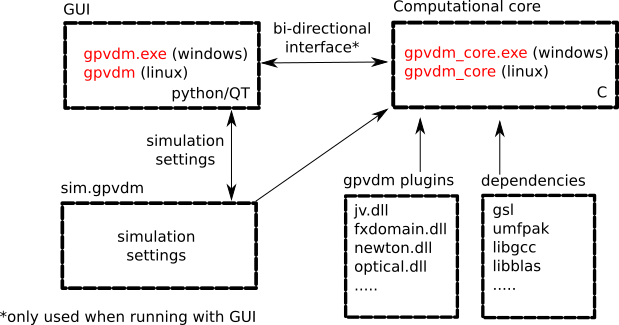
\includegraphics[width=100mm]{./images/architecture.png}
\caption{The structure of the model}
\label{fig:structureofthemodel}
\end{figure}
If you want to run the model from the command line, make a new simulation using the GUI, then close the GUI, and open up the terminal window.  Navigate to the directory where you saved your simulation, then enter C:$\backslash$gpvdm$\backslash$gpvdm\_core.exe in the command line.  gpvdm should then run in the terminal.

\subsection{Structure of the optical model}
I have split the optical model up into different dynamically loadable modules to so that you can write your own optical modules without too much work.  In linux these are .so files and in windows they are .dll files, these are kept in the 'light' directory.  I've not documented the interface of the plugins but if you start looking at light\_interface.c it should be pretty clear.

\subsection{Structure of the electrical solver}
I've broken the electrical model up into various plugins again to make it easier to write extra modules.  They are dynamically loaded as they are needed.  The Newton solvers and matrix inverting libraries are also plugins so they can be swapped out.

\subsection{The materials database and adding new materials}
To calculate the photondensity within the device, the model must know the refractive index and absorption of each material layer.  This data is stored in, C:$\backslash$gpvdm$\backslash$materials.  The subdirectory name in C:$\backslash$gpvdm$\backslash$materials identifies the material name.  In each sub directory there are two key files alpha.omat and n.omat, these files are standard text files can be opened with any text editor such as wordpad.    Alpha.omat contains the absorption coefficient of the material while n.omat contains the the refractive index.  The first column of the file contains the wavelength in $m$ (not $cm$ or $nm$), and the second column of the file contains the absorption coefficient in $m^{-1}$ (for alpha.omat) and the real part of the refractive index (i.e. n) in au (for n.omat).

If you wish to add materials to the database which do not come as standard with the model you can do it in the following way:  Simply copy an existing material directory (say C:$\backslash$gpvdm$\backslash$materials$\backslash$ito) to a new directory (say C:$\backslash$gpvdm$\backslash$materials$\backslash$mynewmaterial).  Then replace alpha.omat and n.omat with your data for the new material. There are two other files in each sub directory, namely fit.inp and mat.inp.  The file fit.inp is needed can be ignored, the file mat.inp is defined as follows:
\newline
\newline
\begin{lstlisting}[language=matlab,frame=single]
#LUMO		The LUMO level of the material 
4.7
#Eg		The LUMO-HOMO level of the material
0.0
#Red		Color of material in GUI
0.4
#Green		Color of material in GUI
0.4
#Blue		Color of material in GUI
0.4
#material_type	Oxide,metal,organic or inorganic.
oxide
#status		Public or private material
public
#ver		The version of the file.
1.0
#end		Defines the end of the file.
\end{lstlisting}

If you don't have data to hand for your material, but you do have a paper containing the data, you use the program Engauge Digitizer, written by  Mark Mitchell \url{https://github.com/markummitchell/engauge-digitizer} to export data from publications.  After you have finished updating the new material directory, whenever a new simulation is generated the new material files will automatically be copied into the active simulation directory ready for use. 

\subsection{Running gpvdm on a cluster}
Gpvdm will run on a cluster, this can be handy when doing large numbers of simulations.  To do this you need to download the cluster management code from  \url{https://github.com/roderickmackenzie/simpleclustercode}.  The clustering code as it stands is pretty much undocumented, but it should be possible to get it going.  You will have to recompile gpvdm to run on the cluster though.

\subsection{Updates}
I suggest you check the webpage regularly for updates, as I often publish minor improvements/bug fixes.  Gpvdm does have a built in update system, when it starts it connects to  \url{http://www.gpvdm.com/download_windows/update.php?ver_core=4.44&os=WinVer}, where 4.44 is replaced by your version of gpvdm and WinVer is replaced by your version of windows.  If no updates are found gpvdm.com will transmit "noupdates" back to the software.  If updates are found, the url will return the text "update 4.45" (where 4.45 is replaced with the most current verstion).  The software will then show a dialog box to inform the user that there is an update available and which version it is.    I've put this feature in, so that if I find a major bug that affects the validity of simulation results, I can inform all users quickly.  The user will then have to go and download it manually to install it.  Currently, there is no option to automatically update the software. 

\subsection{Can I use the model to simulate my exotic* material system/contacts?}
The short answer is yes.  The model is an effective medium model, meaning that it does not simulate the details of the medium, rather it approximates the medium with a set of electrical parameters.  For example, when simulating an organic solar cell, it does not simulate every detail of the BHJ, rather it just assumes an effective mobility, density of states, recombination cross sections, trapping cross sections and so on...  So if you can find electrical parameters to aproximate your material system (or guess them), there is nothing stopping you using gpvdm to simulate any exotic device/material.  The same goes for the contacts, the model simulates the contacts simply as a charge density. So if you have fancy graphene contacts which inject lots of charge, use a high majority carrier density on the contacts.  Where as if you have some dirty old ITO contacts may be drop the majority carrier density a bit.

\section{Installing gpvdm on Linux} \label{installing_on_linux}
The windows version of gpvdm seems to be much more popular than the Linux version.  Therefore, I will tend to publish an updated windows exe every couple of weeks (along with the platform independent source code) and only publish updated linux rpms/deb packages when someone asks me to.  This means that the Linux deb/rpm files tend to lag behind the windows version by about a year.  For this reason I recommend you install the Linux version from source.  If you don't want to do this, drop me an e-mail and I will often be able to push out a new rpm/deb within a day or two.  Currently I provide pre-compiled copies for, Fedora Linux, Ubuntu Linux, Debian Linux, Mint Linux , Opensuse Leap, and Raspbian pi 3.0.


\subsection{Linux from source the easy way}
Make sure you have python3-dialog installed on your system.  Then issue the command ./build in the root directory of gpvdm.  Firstly select (packages) and let the installer install the packages needed to compile gpvdm.  Then select build and let the installer build gpvdm.  You can then exit the installer and run ./gpvdm.  Or if you wish to install gpvdm on your system, chooses install from the menu.

\begin{figure}[ht!]
\centering
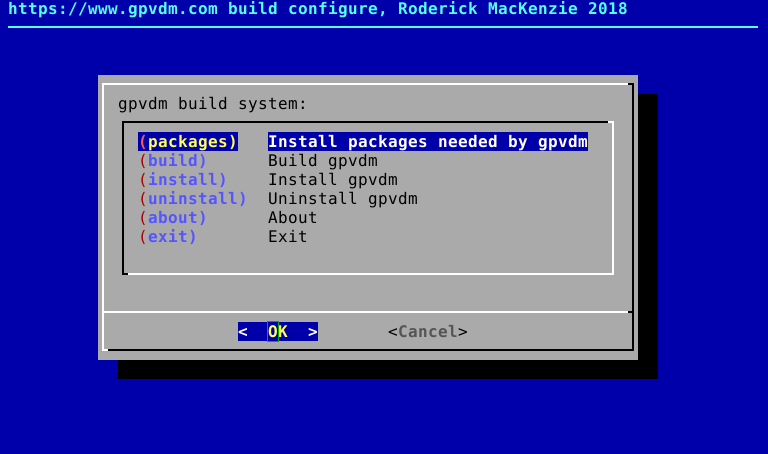
\includegraphics[width=120mm]{./images/build.png}
\caption{The linux build system, run ./build to get this menu.  }
\label{fig:build}
\end{figure}


\subsection{Linux from source the hard way}

On Fedora install the following pacakges:\newline
dnf install zlib-devel libzip-devel libmatheval-devel suitesparse-devel openssl-devel gsl-devel libcurl-devel blas-devel librsvg2-tools texlive ghostscript ImageMagick mencoder valgrind @development-tools fedora-packager mingw32-gcc python-crypto python-awake python3-qt5-devel python3-crypto python3-matplotlib-qt5 python3-openpyxl python3-pyopengl numpy notify-python python-inotify.noarch python-matplotlib python-inotify python-matplotlib indent unifdef indent libcurl-devel poedit ElectricFence kcachegrind help2man\newline
\newline
Then build the build system\newline
aclocal\newline
automake --add-missing\newline
automake\newline
autoconf\newline

Then configure the build system:\newline
./configure CPPFLAGS="-I/usr/include/suitesparse/"\newline

Then make the binary\newline
make\newline
\bibliographystyle{gpvdm.bst}
\bibliography{gpvdm}

\appendix
\addcontentsline{toc}{chapter}{APPENDICES}
\section{Output directories}
\textbf{equilibrium}\newline
Before the solver starts any simulation it solves the device equations in the dark with 0V applied bias.  The result of this calculation are placed in this directory.  The practical reason for doing this is that Newton's method only works if you give it a reasonable starting guess for any given problem.  Thus to start the solver, we guess the carrier densities at 0V in the dark, we then use Newton's method to calculate the exact carrier density profiles at 0V in the dark (results are stored in the equilibrium directory), then from this point we can work our way to other solutions say at +1V in the light.
\newline

\section{Output files}
Writing to disk is slow on even the most modern of computers with an SSD.  The seek speed of mechanical disks has increased little of their history.  Thus often writing the output data to the hard disk is the most time consuming part of any simulation.  By default gpvdm writes all output files to disk.  If you want to speed up your simulation, you can only write the files you need to disk.  This can be done in a fine grained way through the configure window and clicking on the detailed dump control tab.  You will from there be able to turn on and off output files.

\begin{figure}
\centering
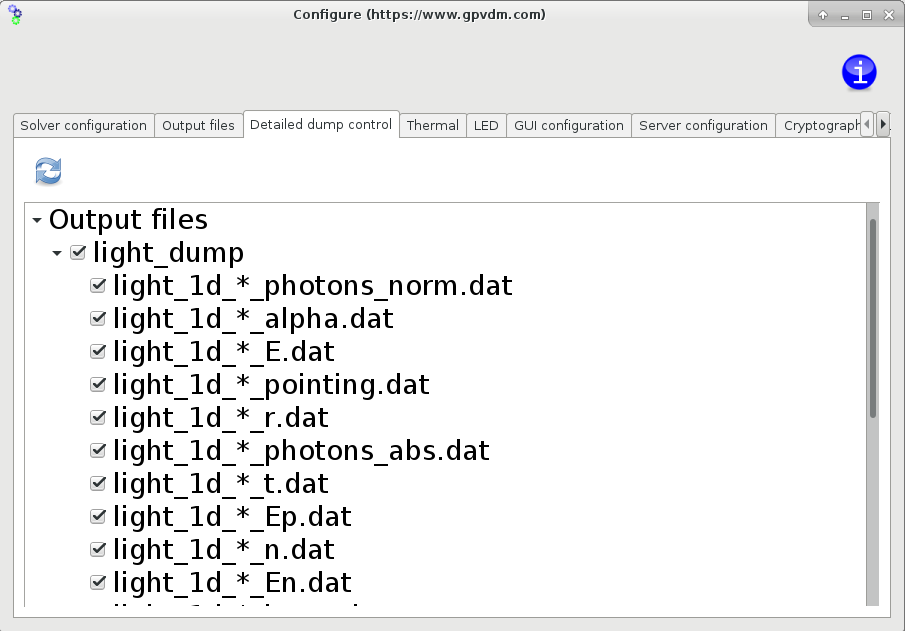
\includegraphics[width=100mm]{./images/output_files.png}
\caption{Selecting which output files are witten to disk.}
\end{figure}

\subsubsection{1D position space output}
\paragraph{Band structure}
\textbf{Ec.dat}:LUMO-position\newline
x-axis:Position($nm$)\newline
y-axis:Electron Energy($eV$)\newline
\newline
\textbf{Efield.dat}:Material number - position\newline
x-axis:Position($nm$)\newline
y-axis:Number($au$)\newline
\newline
\textbf{Eg.dat}:Band gap-position\newline
x-axis:Position($nm$)\newline
y-axis:Electron Energy($eV$)\newline
\newline
\textbf{Ev.dat}:HOMO-position\newline
x-axis:Position($nm$)\newline
y-axis:Electron Energy($eV$)\newline
\newline
\textbf{Fi.dat}:Equlibrium Fermi-level - position\newline
x-axis:Position($nm$)\newline
y-axis:Energy($eV$)\newline
\newline
\textbf{Fn.dat}:Electron quasi Fermi-level position\newline
x-axis:Position($nm$)\newline
y-axis:Electron Energy($eV$)\newline
\newline
\textbf{Fp.dat}:Hole quasi Fermi-level position\newline
x-axis:Position($nm$)\newline
y-axis:Electron Energy($eV$)\newline
\newline
\textbf{phi.dat}:Potential\newline
x-axis:Position($nm$)\newline
y-axis:Potential($V$)\newline
\newline
\paragraph{Chaerge density}
\textbf{dn.dat}:Change in free electron population - position\newline
x-axis:Position($nm$)\newline
y-axis:Carrier density($m^{-3}$)\newline
\newline
\paragraph{Charge density}
\textbf{Nad.dat}:Doping - position\newline
x-axis:Position($nm$)\newline
y-axis:Doping density($m^{-3}$)\newline
\newline
\textbf{dnt.dat}:Excess electron density - position\newline
x-axis:Position($nm$)\newline
y-axis:Electron density($m^{-3}$)\newline
\newline
\textbf{dp.dat}:Change in free hole population - position\newline
x-axis:Position($nm$)\newline
y-axis:Carrier density($m^{-3}$)\newline
\newline
\textbf{dpt.dat}:Excess electron density - position\newline
x-axis:Position($nm$)\newline
y-axis:Hole density($m^{-3}$)\newline
\newline
\textbf{n.dat}:Total hole density - position\newline
x-axis:Position($nm$)\newline
y-axis:Carrier density($m^{-3}$)\newline
\newline
\textbf{nt.dat}:Trapped electron carrier density - position\newline
x-axis:Position($nm$)\newline
y-axis:Carrier density($m^{-3}$)\newline
\newline
\textbf{p.dat}:Total hole density - position\newline
x-axis:Position($nm$)\newline
y-axis:Carrier density($m^{-3}$)\newline
\newline
\textbf{pt.dat}:Trapped hole carrier density - position\newline
x-axis:Position($nm$)\newline
y-axis:Carrier density($m^{-3}$)\newline
\newline
\paragraph{Material parameters}
\textbf{epsilon\_r.dat}:Relative permittivity - position\newline
x-axis:Position($nm$)\newline
y-axis:Relative permittivity($au$)\newline
\newline
\textbf{mu\_n.dat}:Electron mobility - position\newline
x-axis:Position($nm$)\newline
y-axis:Electron mobility($m^{2} V^{-1} s^{-1}$)\newline
\newline
\textbf{mu\_n\_ft.dat}:Electron mobility free/all- position\newline
x-axis:Position($nm$)\newline
y-axis:Mobility($m^{2} V^{-1} s^{-1}$)\newline
\newline
\textbf{mu\_p.dat}:Hole mobility - position\newline
x-axis:Position($nm$)\newline
y-axis:Hole mobility($m^{2} V^{-1} s^{-1}$)\newline
\newline
\textbf{mu\_p\_ft.dat}:Hole mobility free/all- position\newline
x-axis:Position($nm$)\newline
y-axis:Mobility($m^{2} V^{-1} s^{-1}$)\newline
\newline
\textbf{nf.dat}:Free electron carrier density - position\newline
x-axis:Position($nm$)\newline
y-axis:Carrier density($m^{-3}$)\newline
\newline
\textbf{pf.dat}:Free hole carrier density - position\newline
x-axis:Position($nm$)\newline
y-axis:Carrier density($m^{-3}$)\newline
\newline
\paragraph{Model}
\textbf{imat.dat}:Material number - position\newline
x-axis:Position($nm$)\newline
y-axis:Number($au$)\newline
\newline
\paragraph{Recombination}
\textbf{Gn.dat}:Free electron generation rate - position\newline
x-axis:Position($nm$)\newline
y-axis:Generation rate($m^{-3} s^{-1}$)\newline
\newline
\textbf{Gp.dat}:Free hole generation rate - position\newline
x-axis:Position($nm$)\newline
y-axis:Generation rate($m^{-3} s^{-1}$)\newline
\newline
\textbf{Rn\_srh.dat}:SRH electron recombination rate - position\newline
x-axis:Position($nm$)\newline
y-axis:Recombination rate($m^{-3} s^{-1}$)\newline
\newline
\textbf{Rp\_srh.dat}:SRH hole recombination rate - position\newline
x-axis:Position($nm$)\newline
y-axis:Recombination rate($m^{-3} s^{-1}$)\newline
\newline
\textbf{R\_free.dat}:Free electron-hole recombination rate - position\newline
x-axis:Position($nm$)\newline
y-axis:Recombination rate($m^{-3} s^{-1}$)\newline
\newline
\textbf{fsrhh.dat}:Trap fermi level - position\newline
x-axis:Position($nm$)\newline
y-axis:Electron Fermi level($eV$)\newline
\newline
\textbf{fsrhn.dat}:Trap fermi level - position\newline
x-axis:Position($nm$)\newline
y-axis:Electron Fermi level($eV$)\newline
\newline
\textbf{nf\_to\_pt.dat}:Free electron to trapped hole - position\newline
x-axis:Position($nm$)\newline
y-axis:Rate($m^{-3} s^{-1}$)\newline
\newline
\textbf{nrelax.dat}:Electron relaxation rate - position\newline
x-axis:Position($nm$)\newline
y-axis:Rate($m^{-3} s^{-1}$)\newline
\newline
\textbf{pf\_to\_nt.dat}:Free hole to trapped electron - position\newline
x-axis:Position($nm$)\newline
y-axis:Rate($m^{-3} s^{-1}$)\newline
\newline
\textbf{prelax.dat}:Hole relaxation rate - position\newline
x-axis:Position($nm$)\newline
y-axis:Rate($m^{-3} s^{-1}$)\newline
\newline

\textbf{Photon\_gen.dat}:Photon generation rate - position\newline
x-axis:Position($nm$)\newline
y-axis:Photon generation rate($m^{-3} s^{-1}$)\newline

\paragraph{Transport}
\textbf{Jn.dat}:Current density - position\newline
x-axis:Position($nm$)\newline
y-axis:Electron current density($A m^{-2}$)\newline
\newline
\textbf{Jn\_diffusion.dat}:Diffusion current density - position\newline
x-axis:Position($nm$)\newline
y-axis:Electron current density (diffusion)($A m^{-2}$)\newline
\newline
\textbf{Jn\_drift.dat}:Drift current density - position\newline
x-axis:Position($nm$)\newline
y-axis:Electron current density (drift)($A m^{-2}$)\newline
\newline
\textbf{Jn\_plus\_Jp.dat}:Total current density (Jn+Jp) - position\newline
x-axis:Position($nm$)\newline
y-axis:Total current density (Jn+Jp)($A m^{-2}$)\newline
\newline
\textbf{Jp.dat}:Current density - position\newline
x-axis:Position($nm$)\newline
y-axis:Hole current density($A m^{-2}$)\newline
\newline
\textbf{Jp\_diffusion.dat}:Diffusion current density - position\newline
x-axis:Position($nm$)\newline
y-axis:Hole current density (diffusion)($A m^{-2}$)\newline
\newline
\textbf{Jp\_drift.dat}:Drift current density - position\newline
x-axis:Position($nm$)\newline
y-axis:Hole current density (drift)($A m^{-2}$)\newline
\newline
\textbf{Jp\_drift\_plus\_diffusion.dat}:Total current density (Jn+Jp) - position\newline
x-axis:Position($nm$)\newline
y-axis:Total current density (Jn+Jp)($A m^{-2}$)\newline
\newline


\end{document}

